\section{Corrections on MC} \label{CorrectionsOnMC}

\subsection{Luminosity Scale factors}

The number of generated MC events listed on tables \ref{tab:BkgList2016}, \ref{tab:BkgList2017},
and \ref{tab:BkgList2018} are arbitrary. In order to compare it with data, the
former has to be rescaled to account for the amount of data collected each year
during the data taking period. The luminosity scale factor is computed as follows:

\begin{equation}
  L_{sf}=\frac{L_{\rm data}}{L_{\rm MC}} = \frac{L_{\rm data}\times\sigma_{\rm MC}}{n_{\rm MC}},
\label{eq:lumiSF}
\end{equation}

Where $L_{\rm data}$ is the luminosity per year, see table \ref{tab:LuminosityPerYear},
$n_{MC}$ the number of generated MC events as provided by the sum of weighted events
from the generator (\verb|genWeight| branch on \verb|NanoAOD|), and $\sigma_{\rm MC}$
is the cross section of the MC samples as provided by \verb|XSecAnalyzer|.

\subsection{K-Factor}

\begin{figure}[tph]
  \centering
  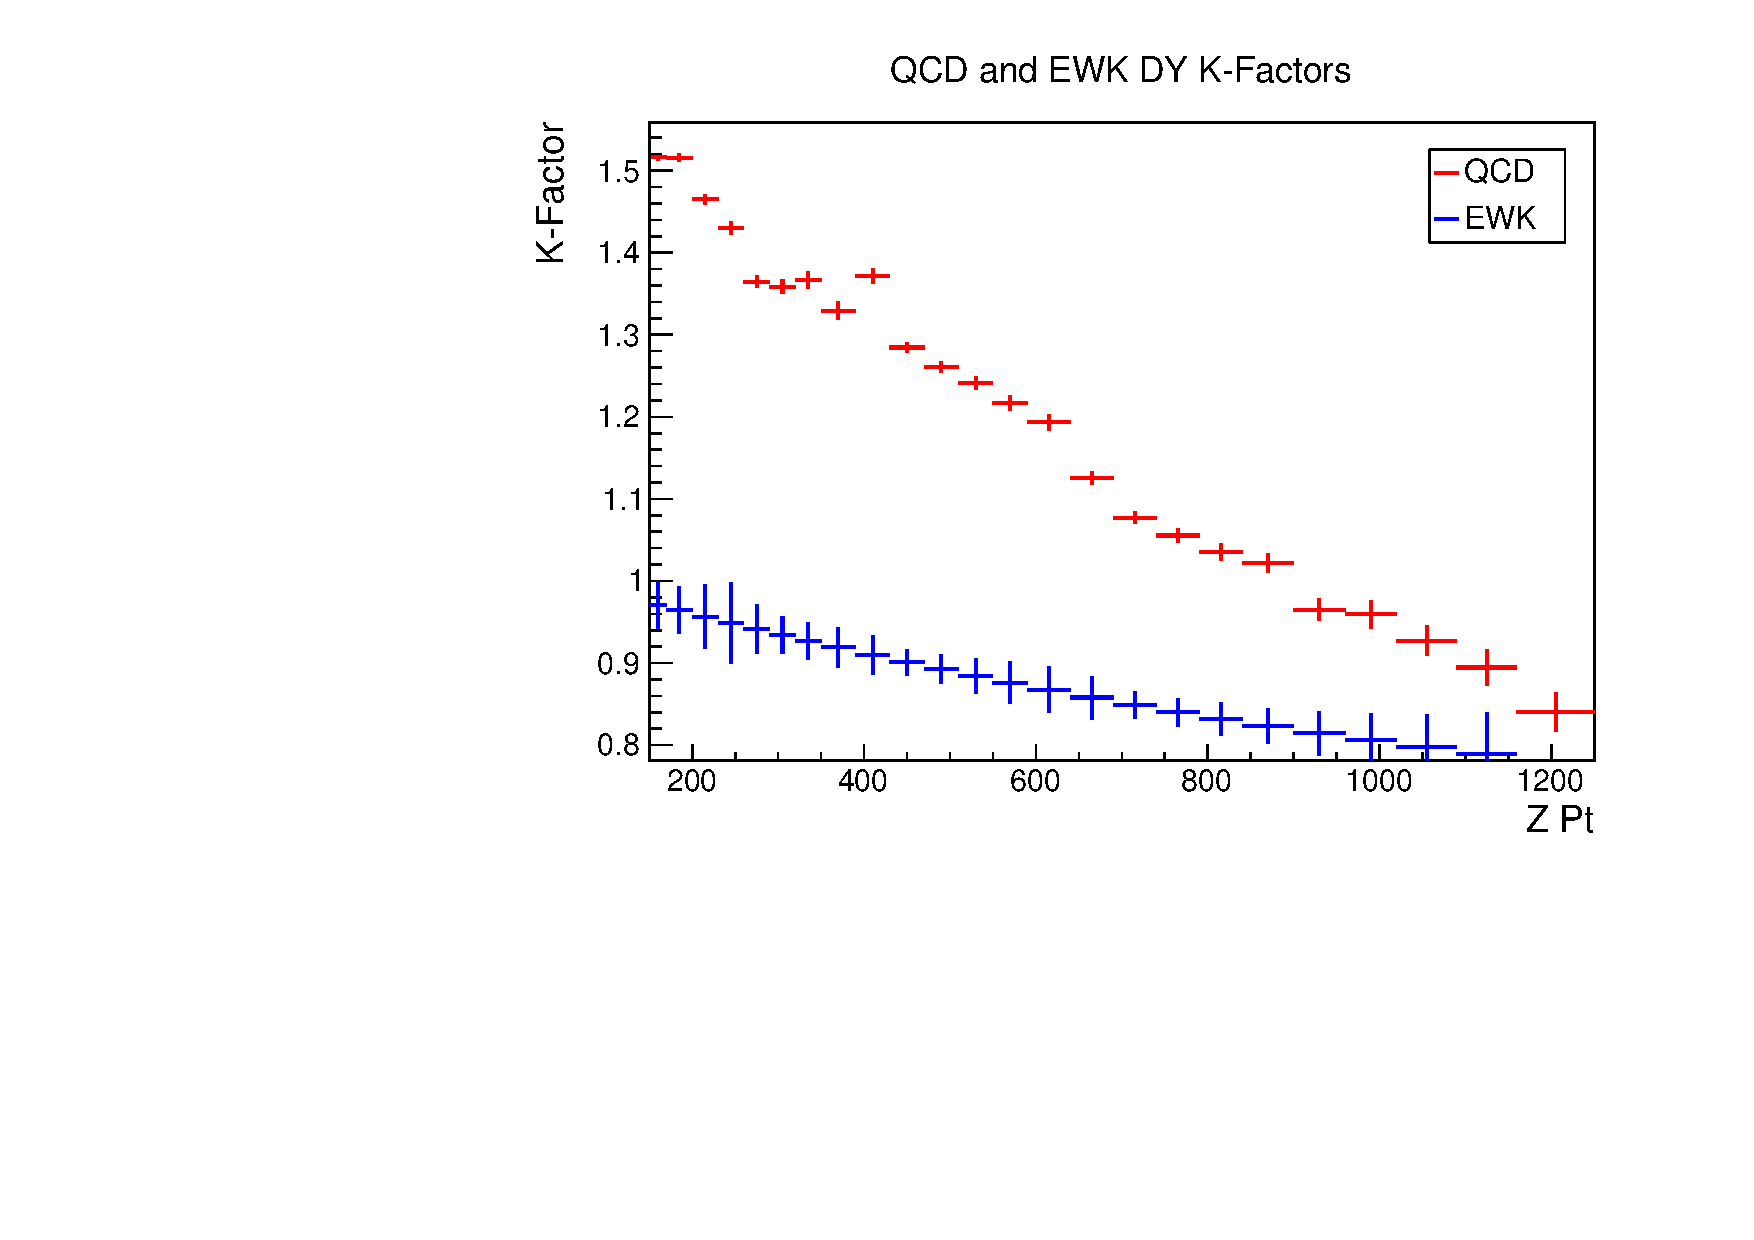
\includegraphics[width=0.6\textwidth]{fig/ScaleFactors/QCD_EWK_DYKFactors.pdf}
  \caption{QCD and Electroweak k-Factors as a function of the Z boson's transverse
   momentum
  }
  \label{fig:kFactors}
\end{figure}

Next-to-leading order QCD and Electroweak (EWK) corrections to the Drell-Yan
process are applied as a function of the reconstructed Z boson.


\subsection{Pileup Reweighting}

\begin{figure}[tph]
  \centering
        \subfigure[Standard model WZ production normalized pileup distributions for Run 2 years]{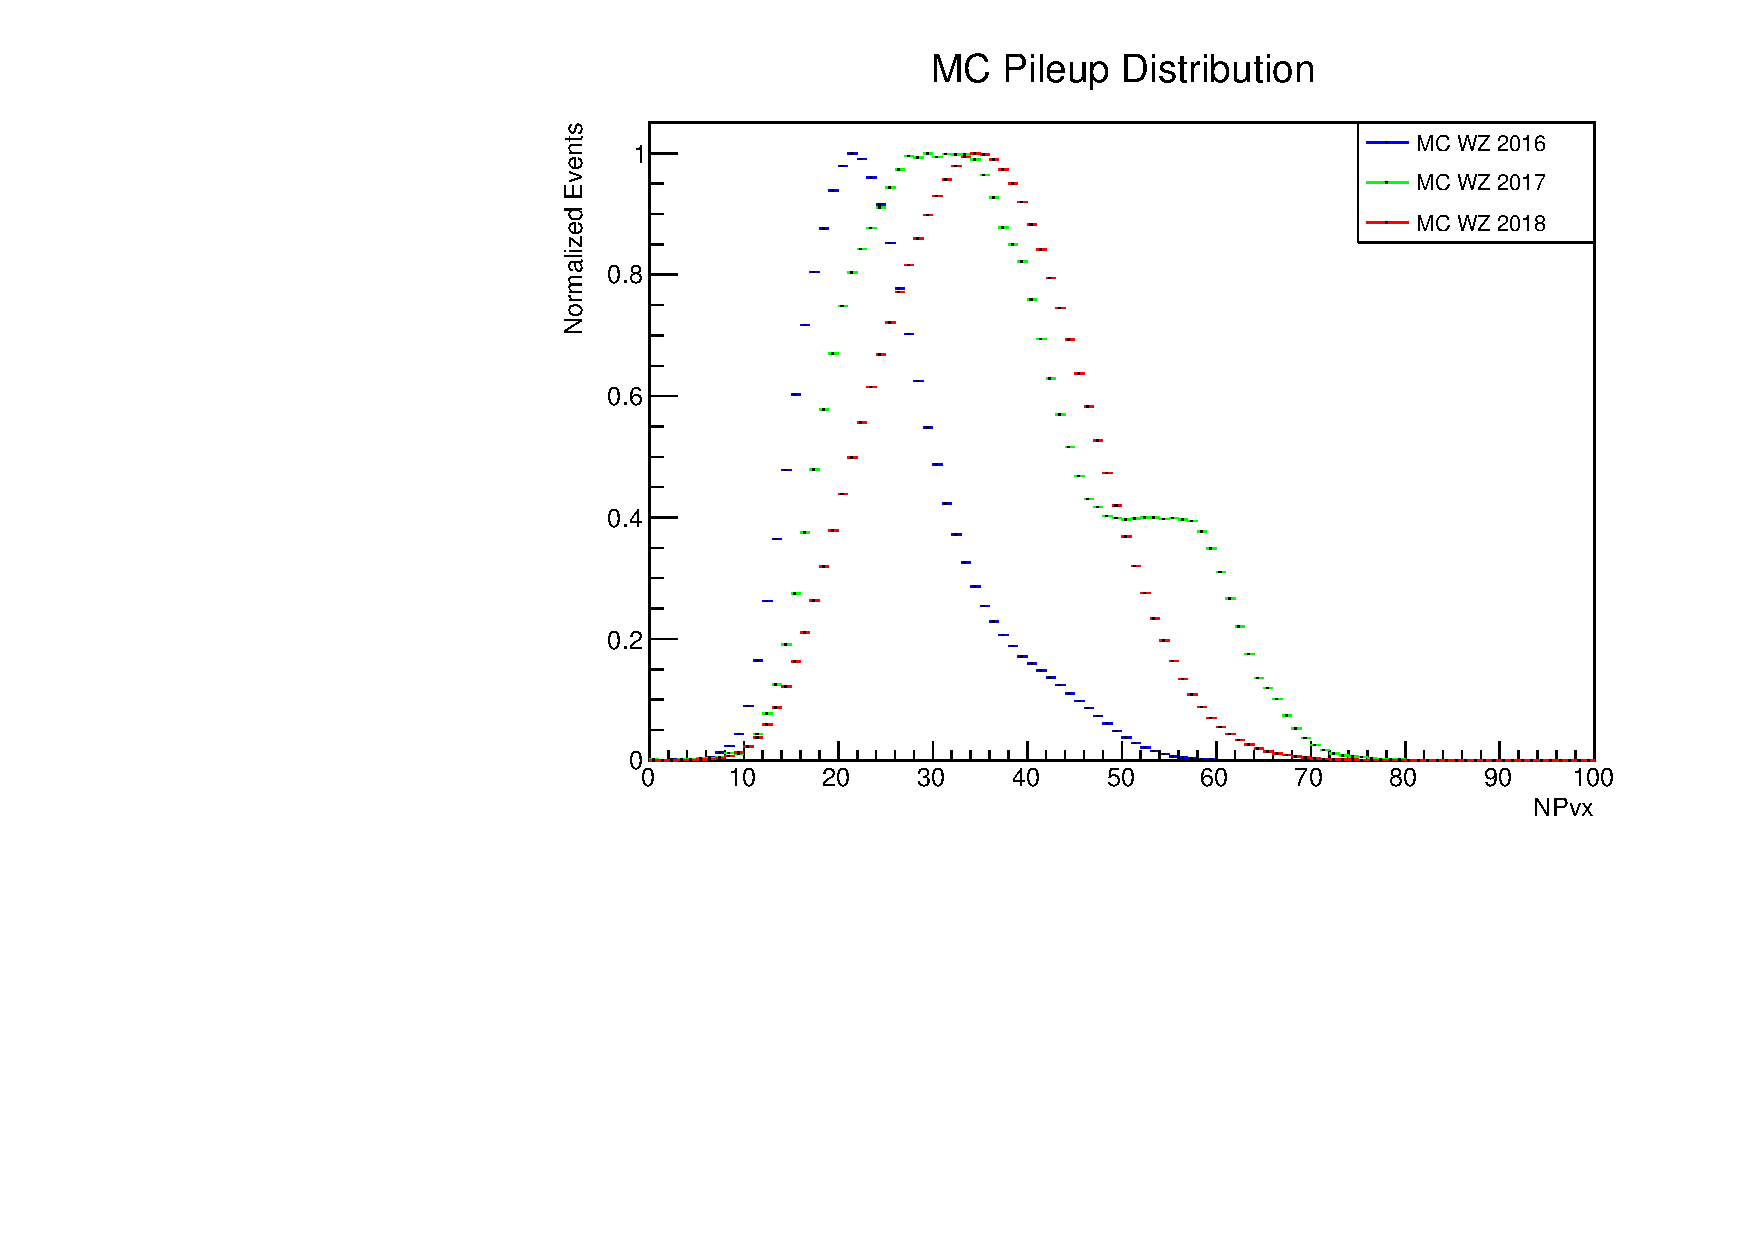
\includegraphics[width=.5\textwidth]{fig/ScaleFactors/MC_Pileup_Linear.pdf}}
        \subfigure[Pileup profile from Run 2 Data, Linear Scale]{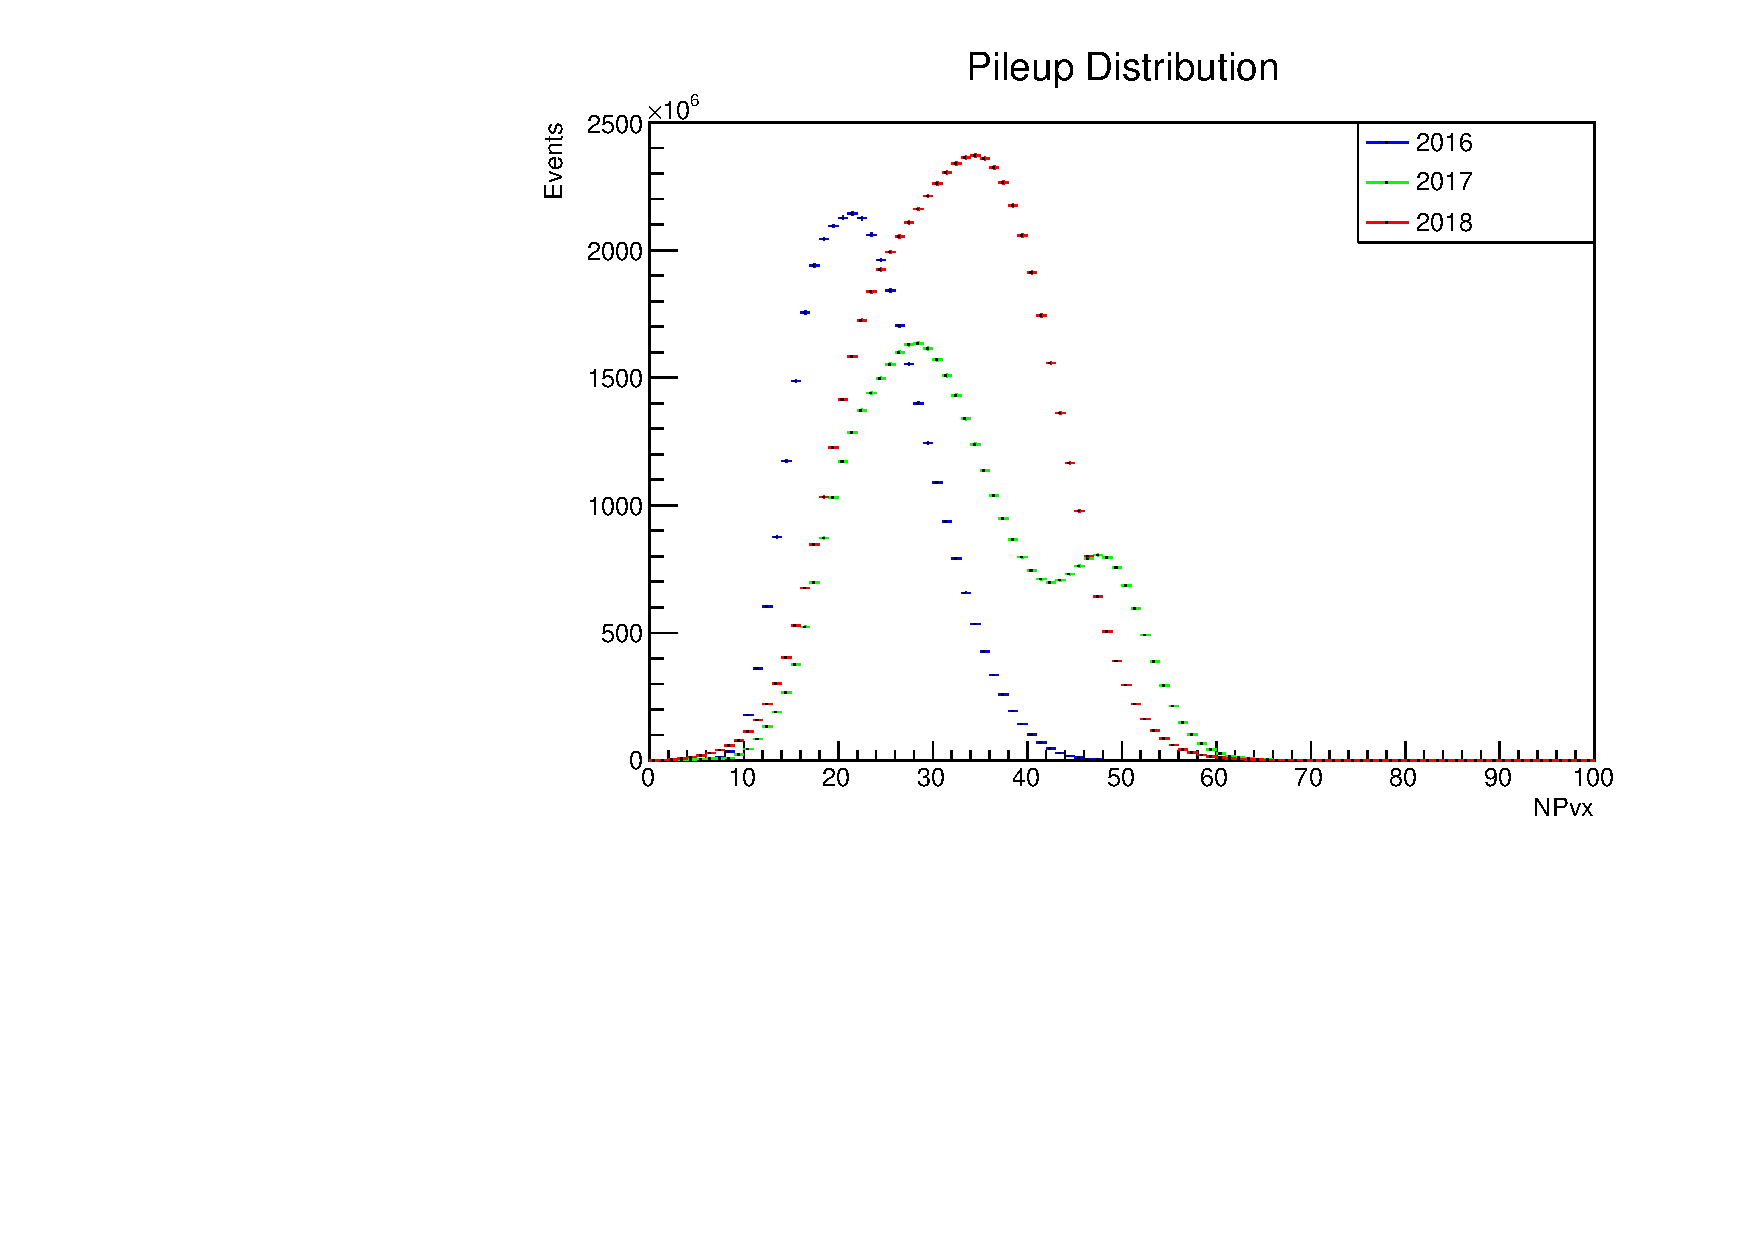
\includegraphics[width=.5\textwidth]{fig/ScaleFactors/GoldenPileup_Linear.pdf}}
        \vfil
        \subfigure[Pileup profile from Run 2 Data, Logarithmic Scale]{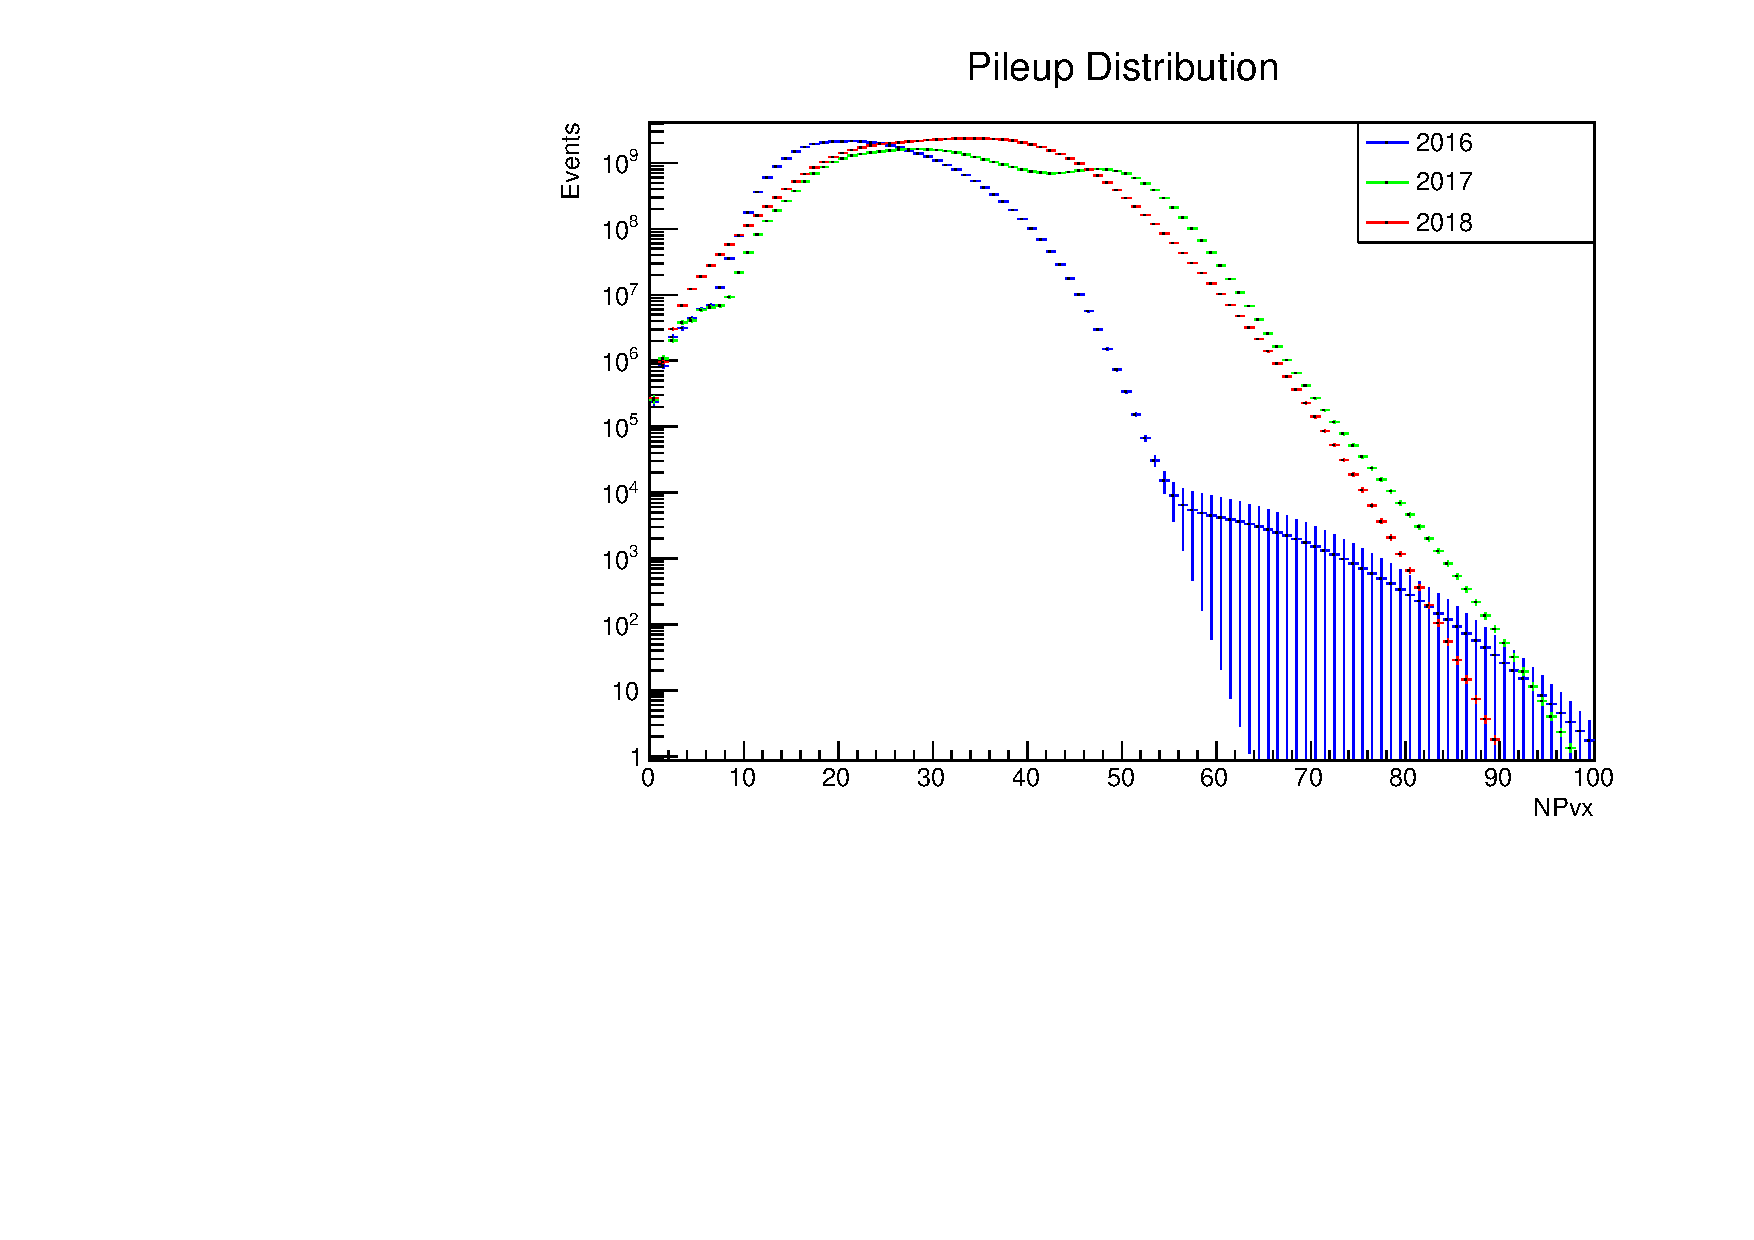
\includegraphics[width=.5\textwidth]{fig/ScaleFactors/GoldenPileup_LogScale.pdf}}
        \subfigure[Pileup weight profiles for several background samples]{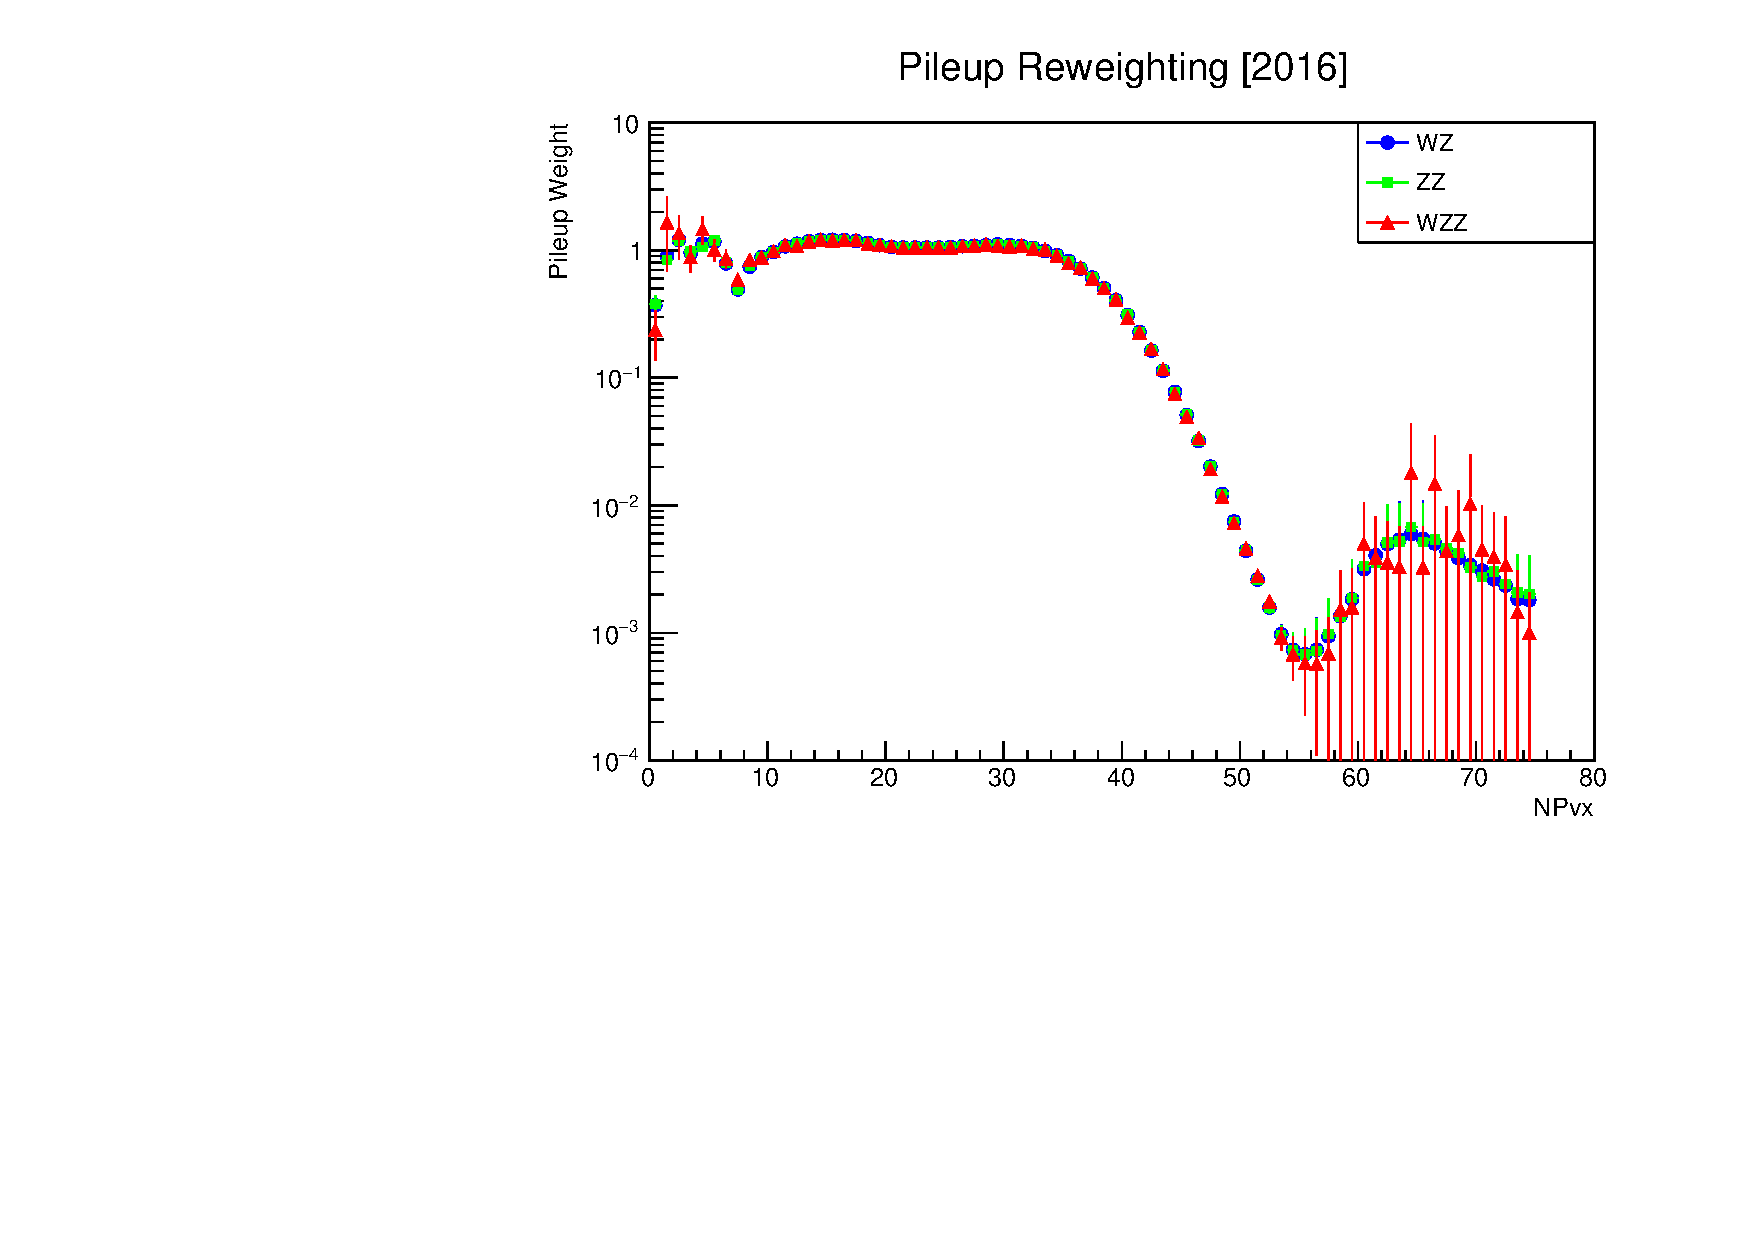
\includegraphics[width=.5\textwidth]{fig/ScaleFactors/PileupWeight_LogScale.pdf}}
  \caption{Pileup profile distributions for MC and Data}
  \label{fig:RunII_PileupProfiles}
\end{figure}

The number of reconstructed primary vertices in each collision during a period
of time generates a distribution commonly referred as pileup. Montecarlo simulations
are produced with an estimated pileup profile and a correction is needed
in order to match the distributions obtained in the collected data.
MC Samples are reweighted with $69.2~mb$ as MinBias cross section \cite{pureweight}.
Figure \ref{fig:RunII_PileupProfiles} shows the differences between the
pileup distributions for run 2 data and montecarlo
simulations for the predominant background process (standard model
WZ production). These differences are then
corrected by computing a pileup weight bin by bin that matches the normalized
distribution from montecarlo with the normalized distribution from data.
The normalization of each distribution is eachieved by scaling it by a factor
equivalent to the the inverse of its integral. Each MC event is then reweighted
with the appropiate factor based on the number of reconstructed primary vertices. 

\subsection{Lepton scale factors}

\begin{figure}[tph]
  \centering
  \subfigure[Electron Loose ID. Applied to the $eee$ and $ee\mu$ channels
    based on the pseudorapidity $\eta$ and transverse momentum $P_{t}$ of each
    of the electrons used to define a $Z$ candidate in the event.
    The applied weight is the product of the scale factors of each individual electron.
  ]{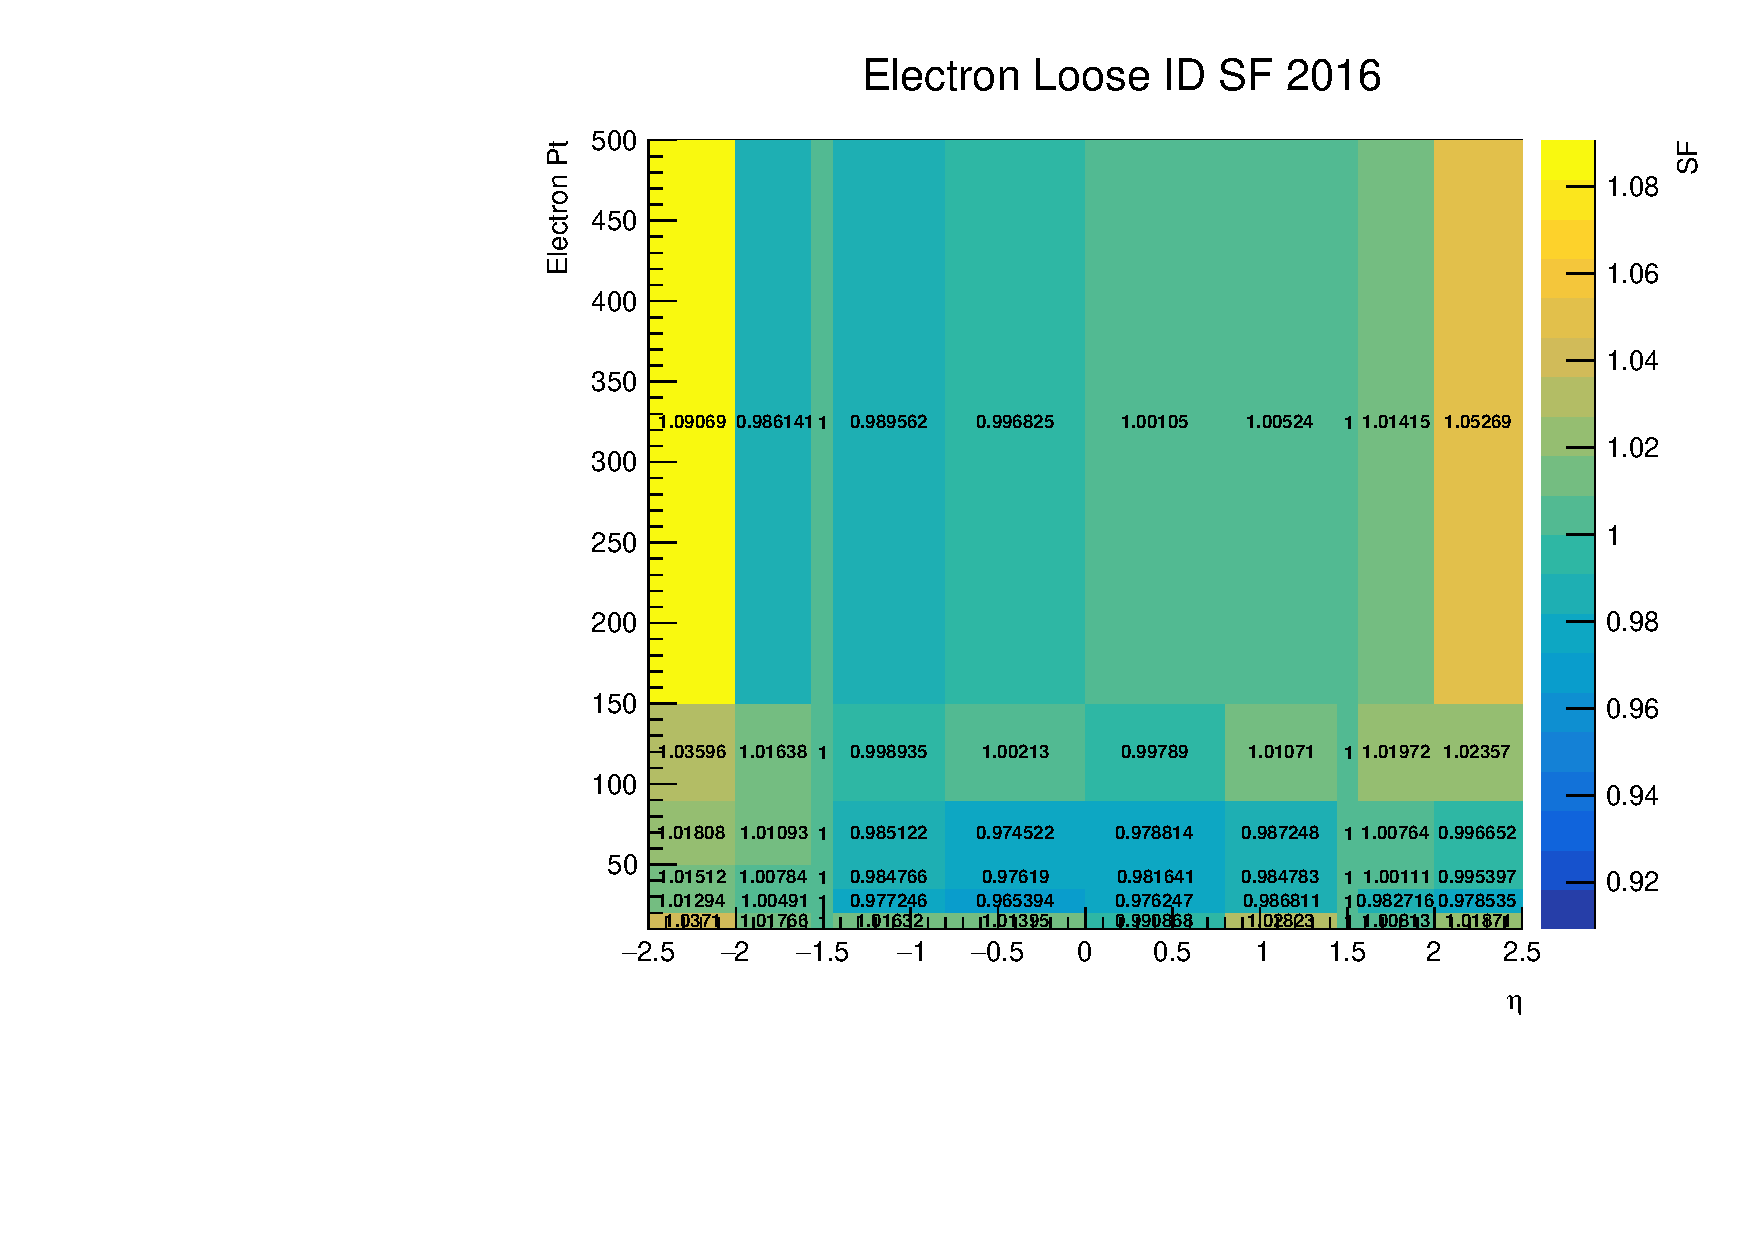
\includegraphics[width=.45\textwidth]{fig/ScaleFactors/2016Electron_LooseID.pdf}}
  \hspace{5mm}
  \subfigure[Electron Tight ID. Applied to the $eee$ and $\mu\mu e$ channels
    based on the pseudorapidity $\eta$ and transverse momentum $P_{t}$ of the
    electron used to define the $W$ candidate.
  ]{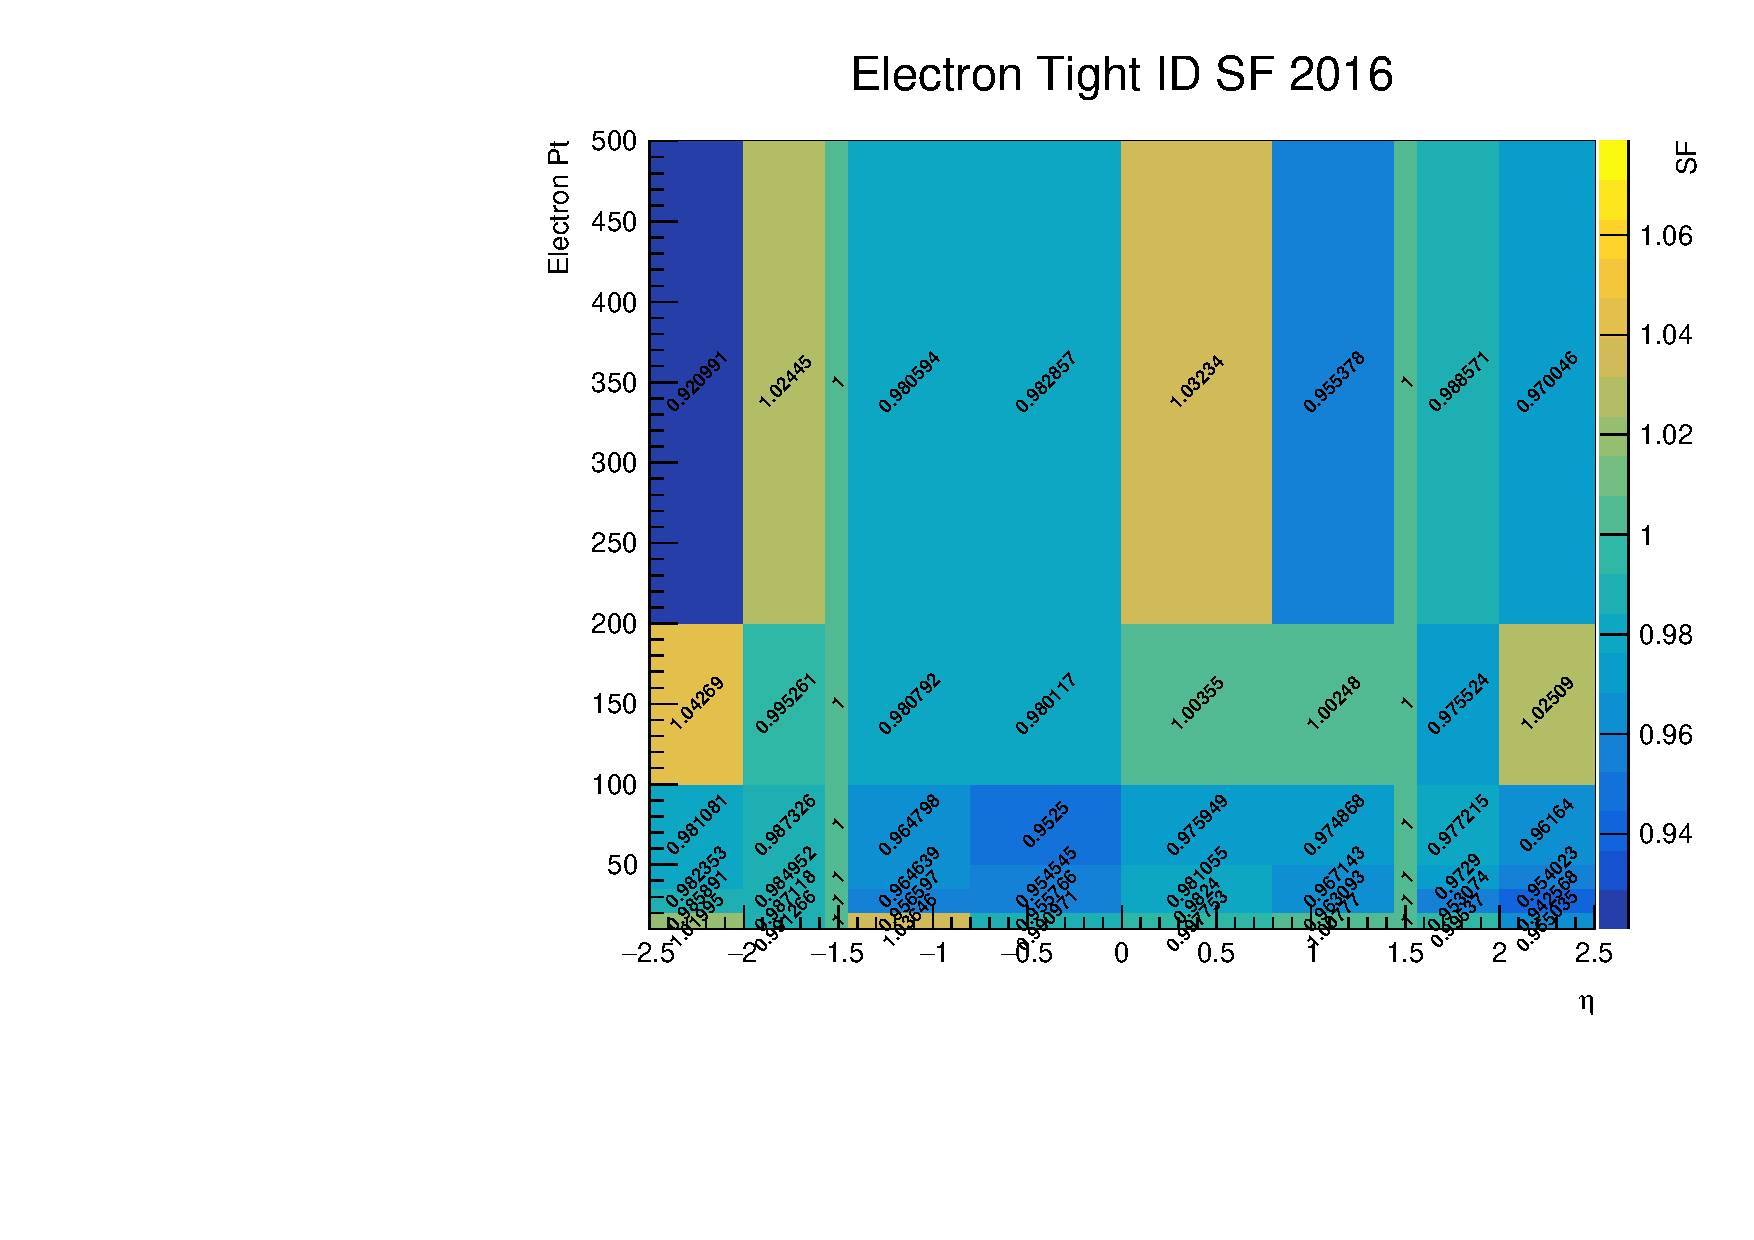
\includegraphics[width=.45\textwidth]{fig/ScaleFactors/2016Electron_TightID.pdf}}
  \vfil
  \subfigure[Muon GlobalHighPtId. Applied to the $\mu\mu e$, $ee\mu$,
    and $\mu\mu\mu$ channels based on the pseudorapidity $\eta$ and transverse
    momentum $P_{t}$ of each of the muons used to define a $WZ$ candidate in the event
    identified as GlobalHighPt.
    The applied weight is the product of the scale factors of each individual muon.
  ]{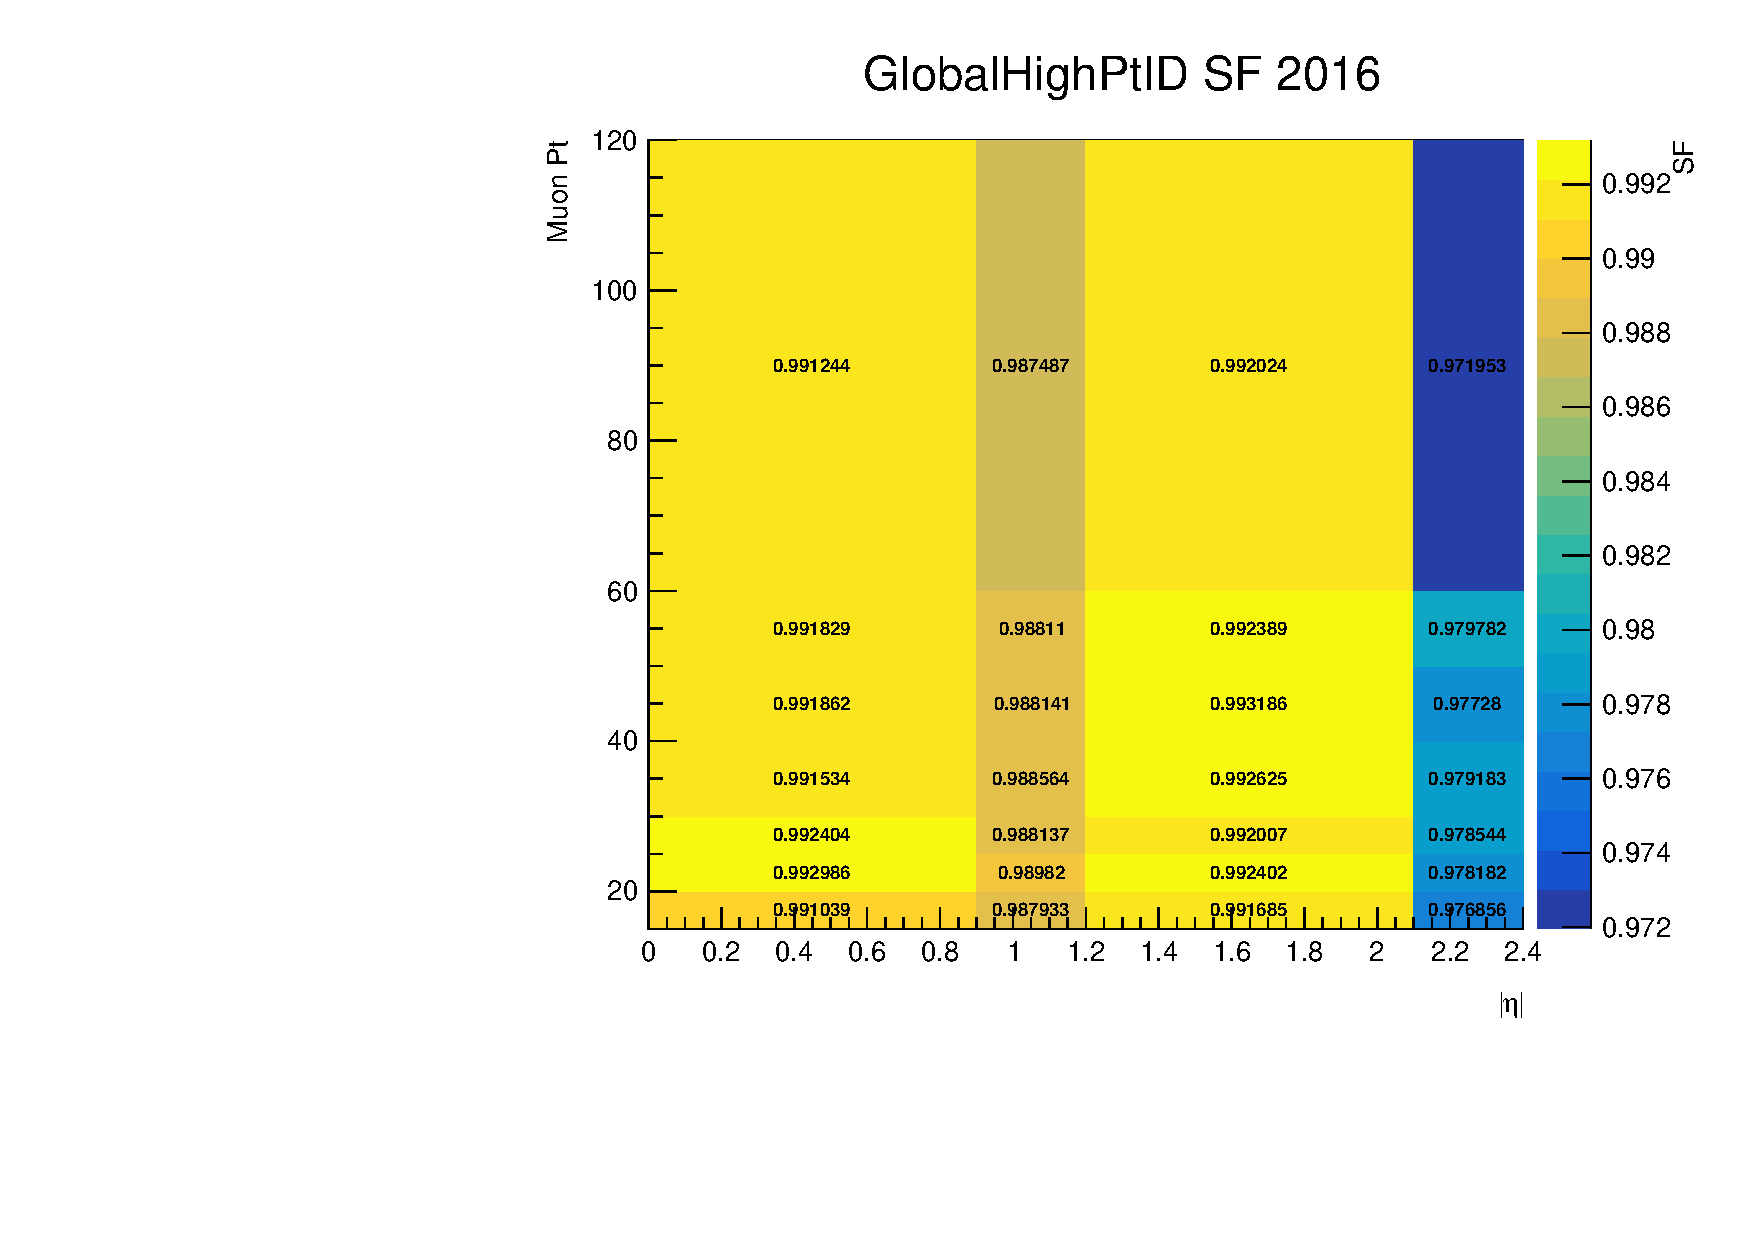
\includegraphics[width=.45\textwidth]{fig/ScaleFactors/2016Muon_GlobalHighPtID.pdf}}
  \hspace{5mm}
  \subfigure[Muon TrkHighPtId. Applied to the $\mu\mu e$ and $ee\mu$,
     and $\mu\mu\mu$ channels based on the pseudorapidity $\eta$ and transverse
     momentum $P_{t}$ of each of the muons used to define a $WZ$ candidate in the event
     identified as TrackerHighPt.
     The applied weight is the product of the scale factors of each individual muon.
  ]{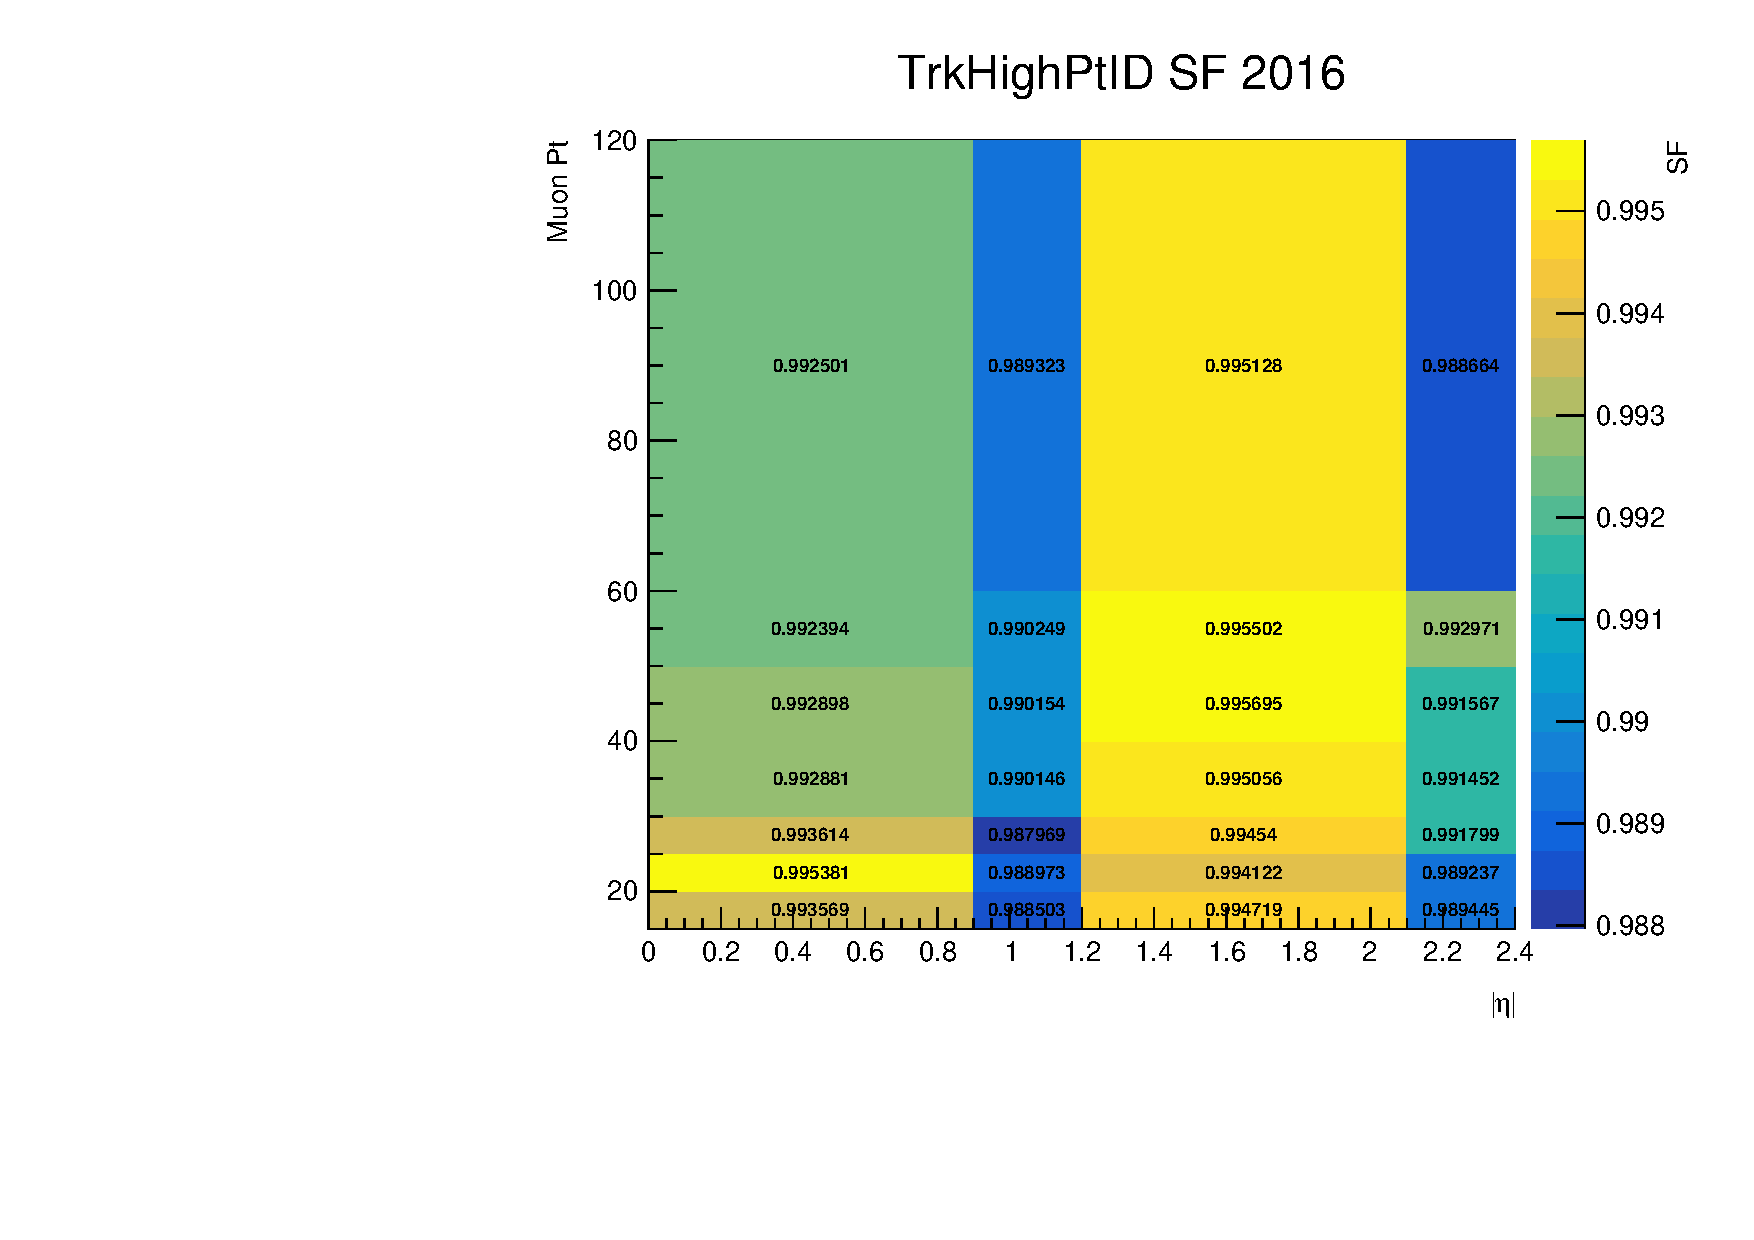
\includegraphics[width=.45\textwidth]{fig/ScaleFactors/2016Muon_TrkHighPtID.pdf}}
  \caption{Lepton ID Scale Factors 2016}
  \label{fig:leptonidsf_2016}
\end{figure}

\begin{figure}[tph]
  \centering
  \subfigure[Electron Loose ID. Applied to the $eee$ and $ee\mu$ channels
    based on the pseudorapidity $\eta$ and transverse momentum $P_{t}$ of each
    of the electrons used to define a $Z$ candidate in the event.
    The applied weight is the product of the scale factors of each individual electron.
  ]{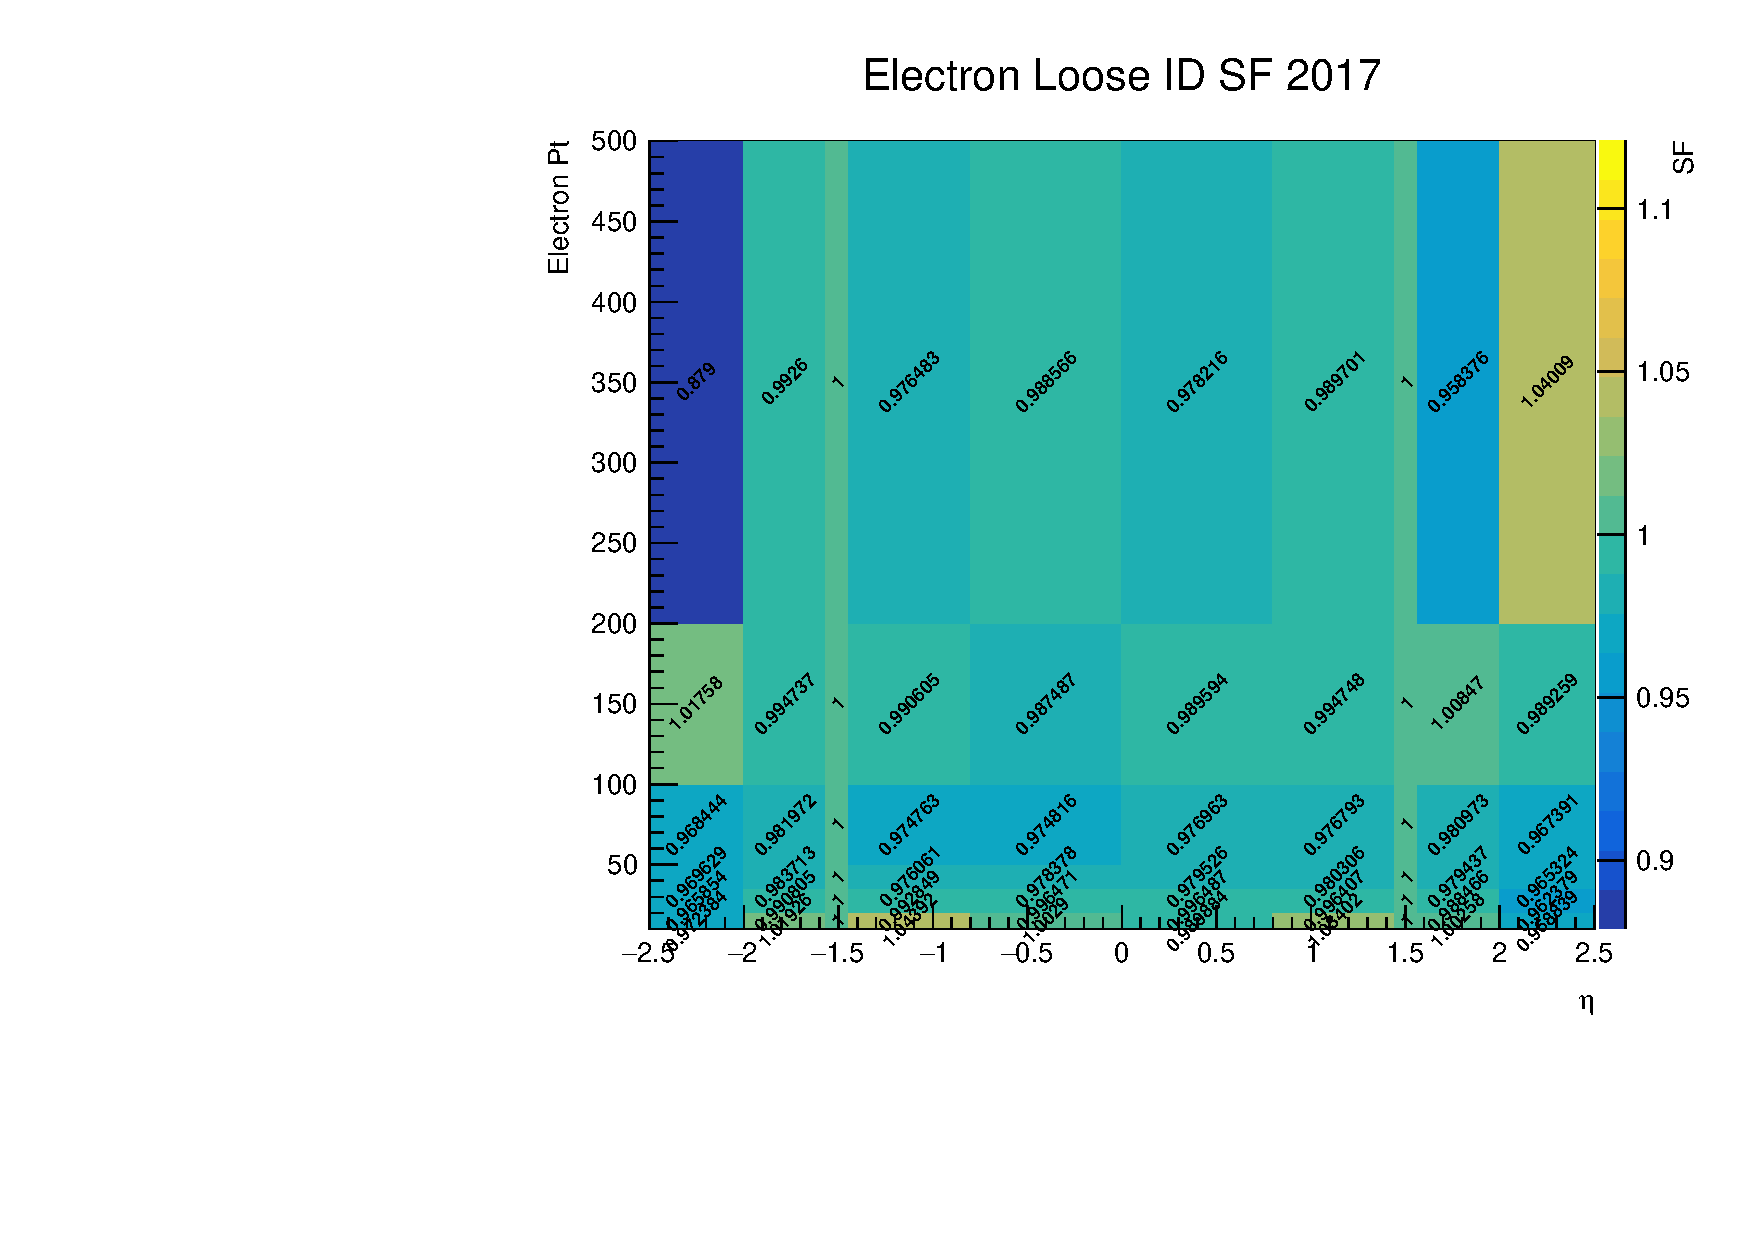
\includegraphics[width=.45\textwidth]{fig/ScaleFactors/2017Electron_LooseID.pdf}}
  \hspace{5mm}
  \subfigure[Electron Tight ID. Applied to the $eee$ and $\mu\mu e$ channels
    based on the pseudorapidity $\eta$ and transverse momentum $P_{t}$ of the
    electron used to define the $W$ candidate.]{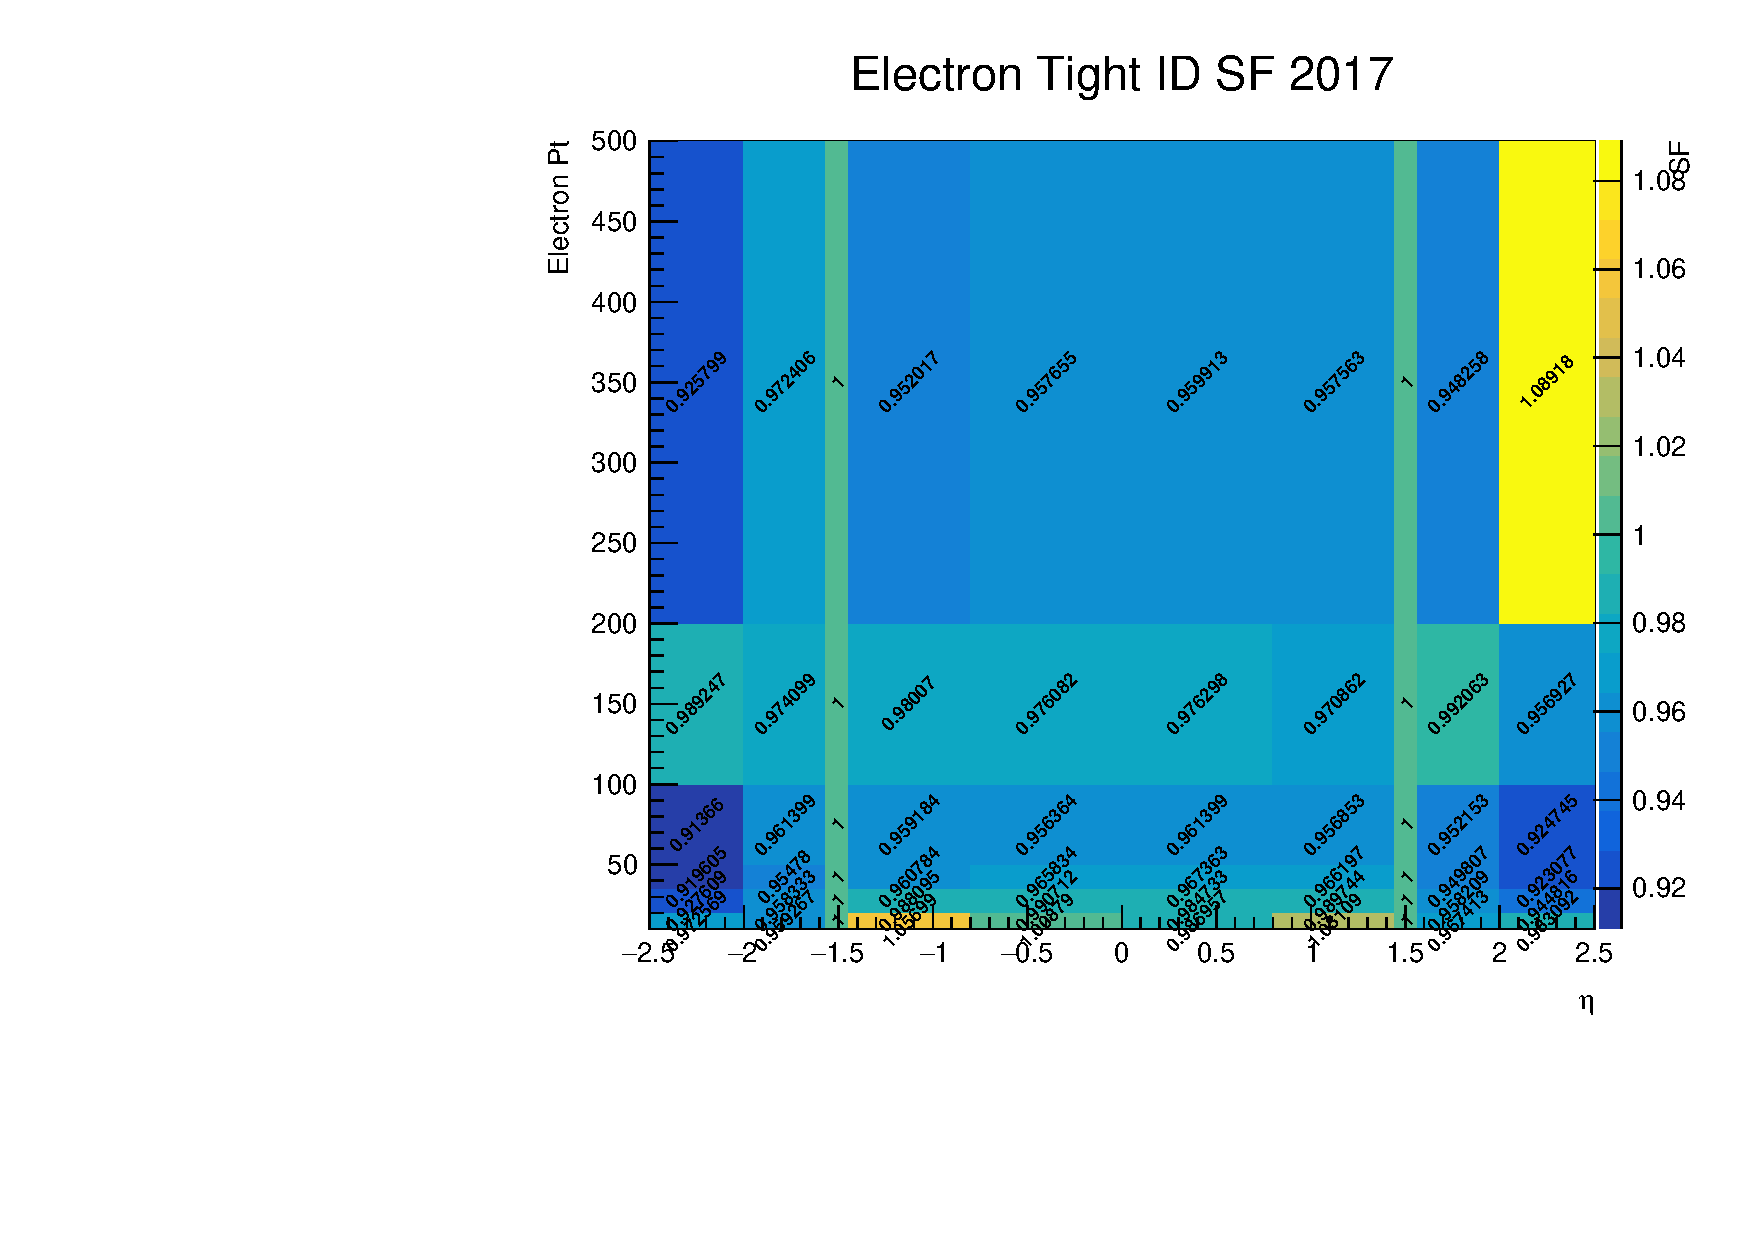
\includegraphics[width=.45\textwidth]{fig/ScaleFactors/2017Electron_TightID.pdf}}
  \vfil
  \subfigure[Muon GlobalHighPtId. Applied to the $\mu\mu e$, $ee\mu$,
    and $\mu\mu\mu$ channels based on the pseudorapidity $\eta$ and transverse
    momentum $P_{t}$ of each of the muons used to define a $WZ$ candidate in the event
    identified as GlobalHighPt.
    The applied weight is the product of the scale factors of each individual muon.
  ]{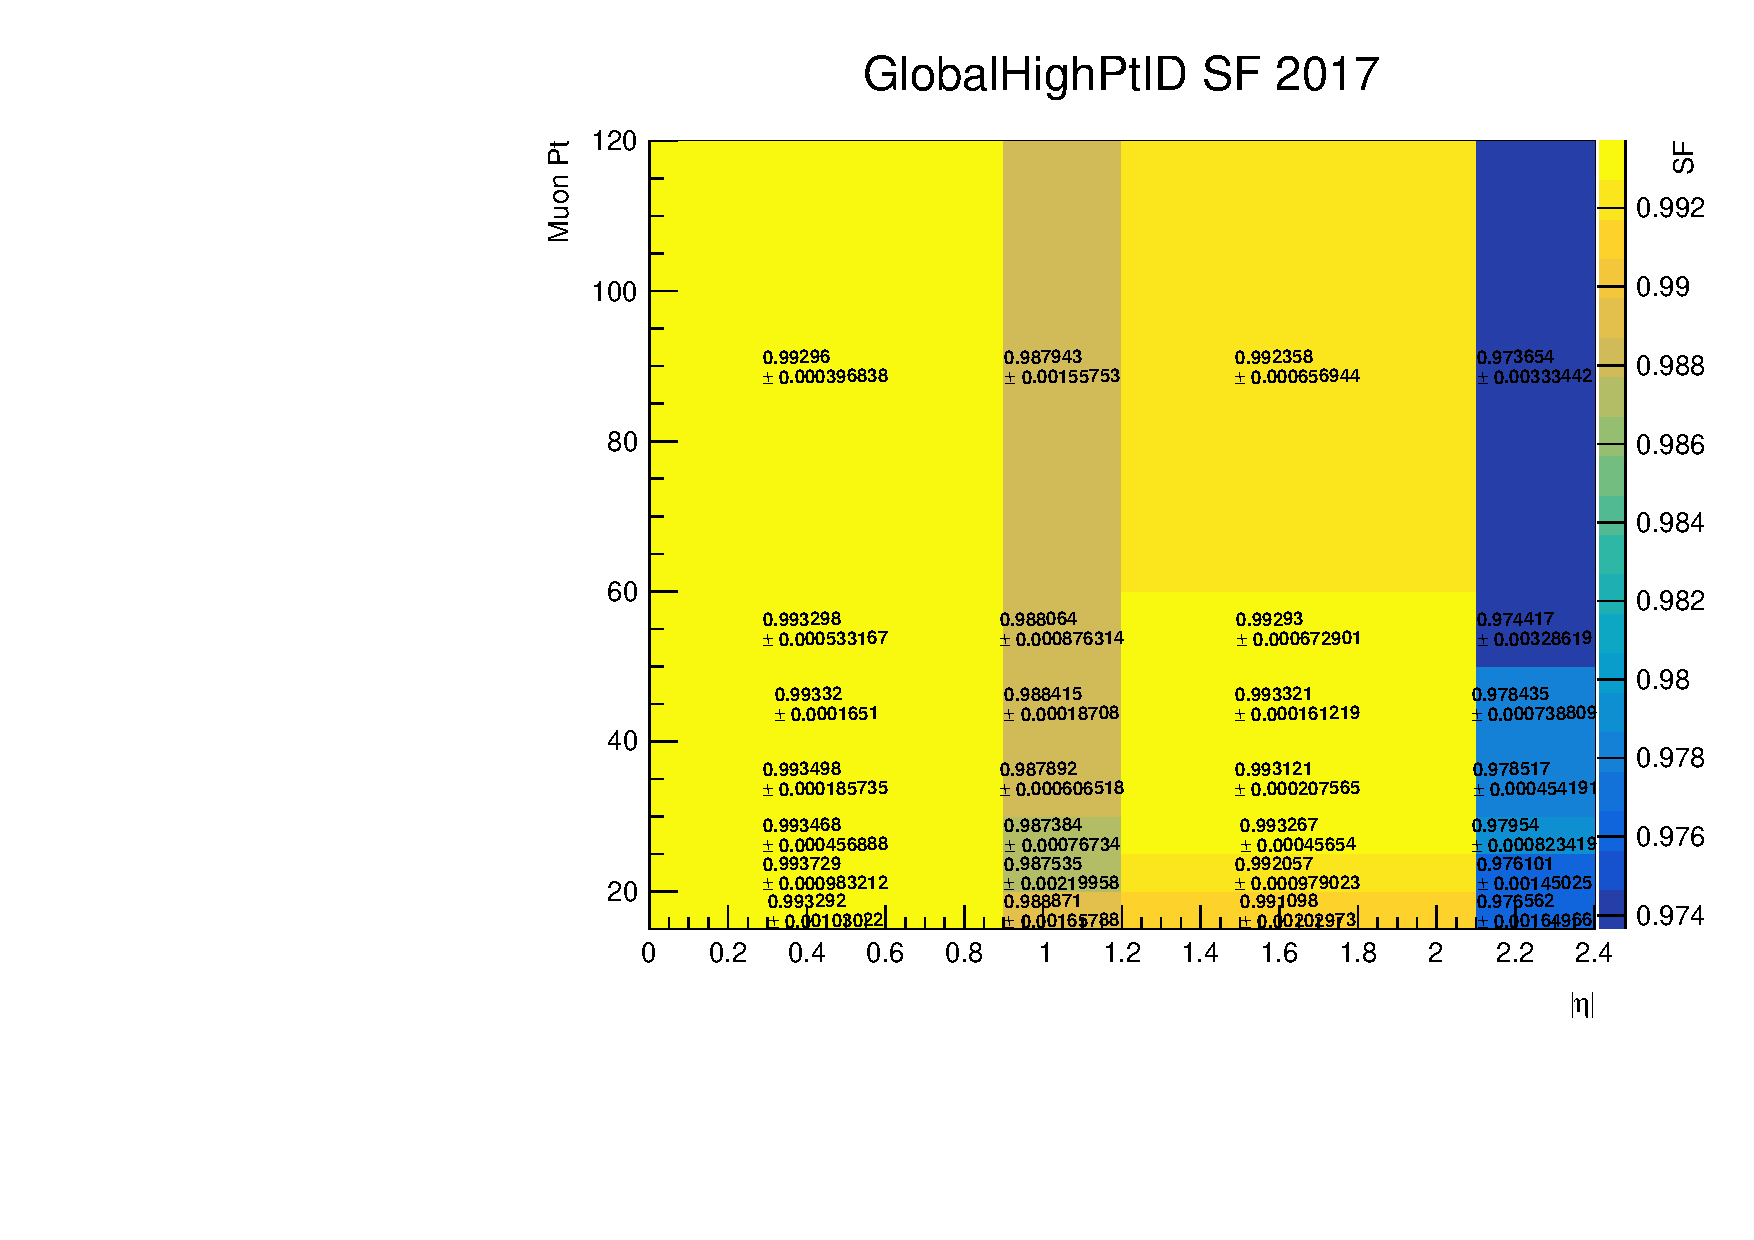
\includegraphics[width=.45\textwidth]{fig/ScaleFactors/2017Muon_GlobalHighPtID.pdf}}
  \hspace{5mm}
  \subfigure[Muon TrkHighPtId. Applied to the $\mu\mu e$ and $ee\mu$,
     and $\mu\mu\mu$ channels based on the pseudorapidity $\eta$ and transverse
     momentum $P_{t}$ of each of the muons used to define a $WZ$ candidate in the event
     identified as TrackerHighPt.
    The applied weight is the product of the scale factors of each individual muon.
  ]{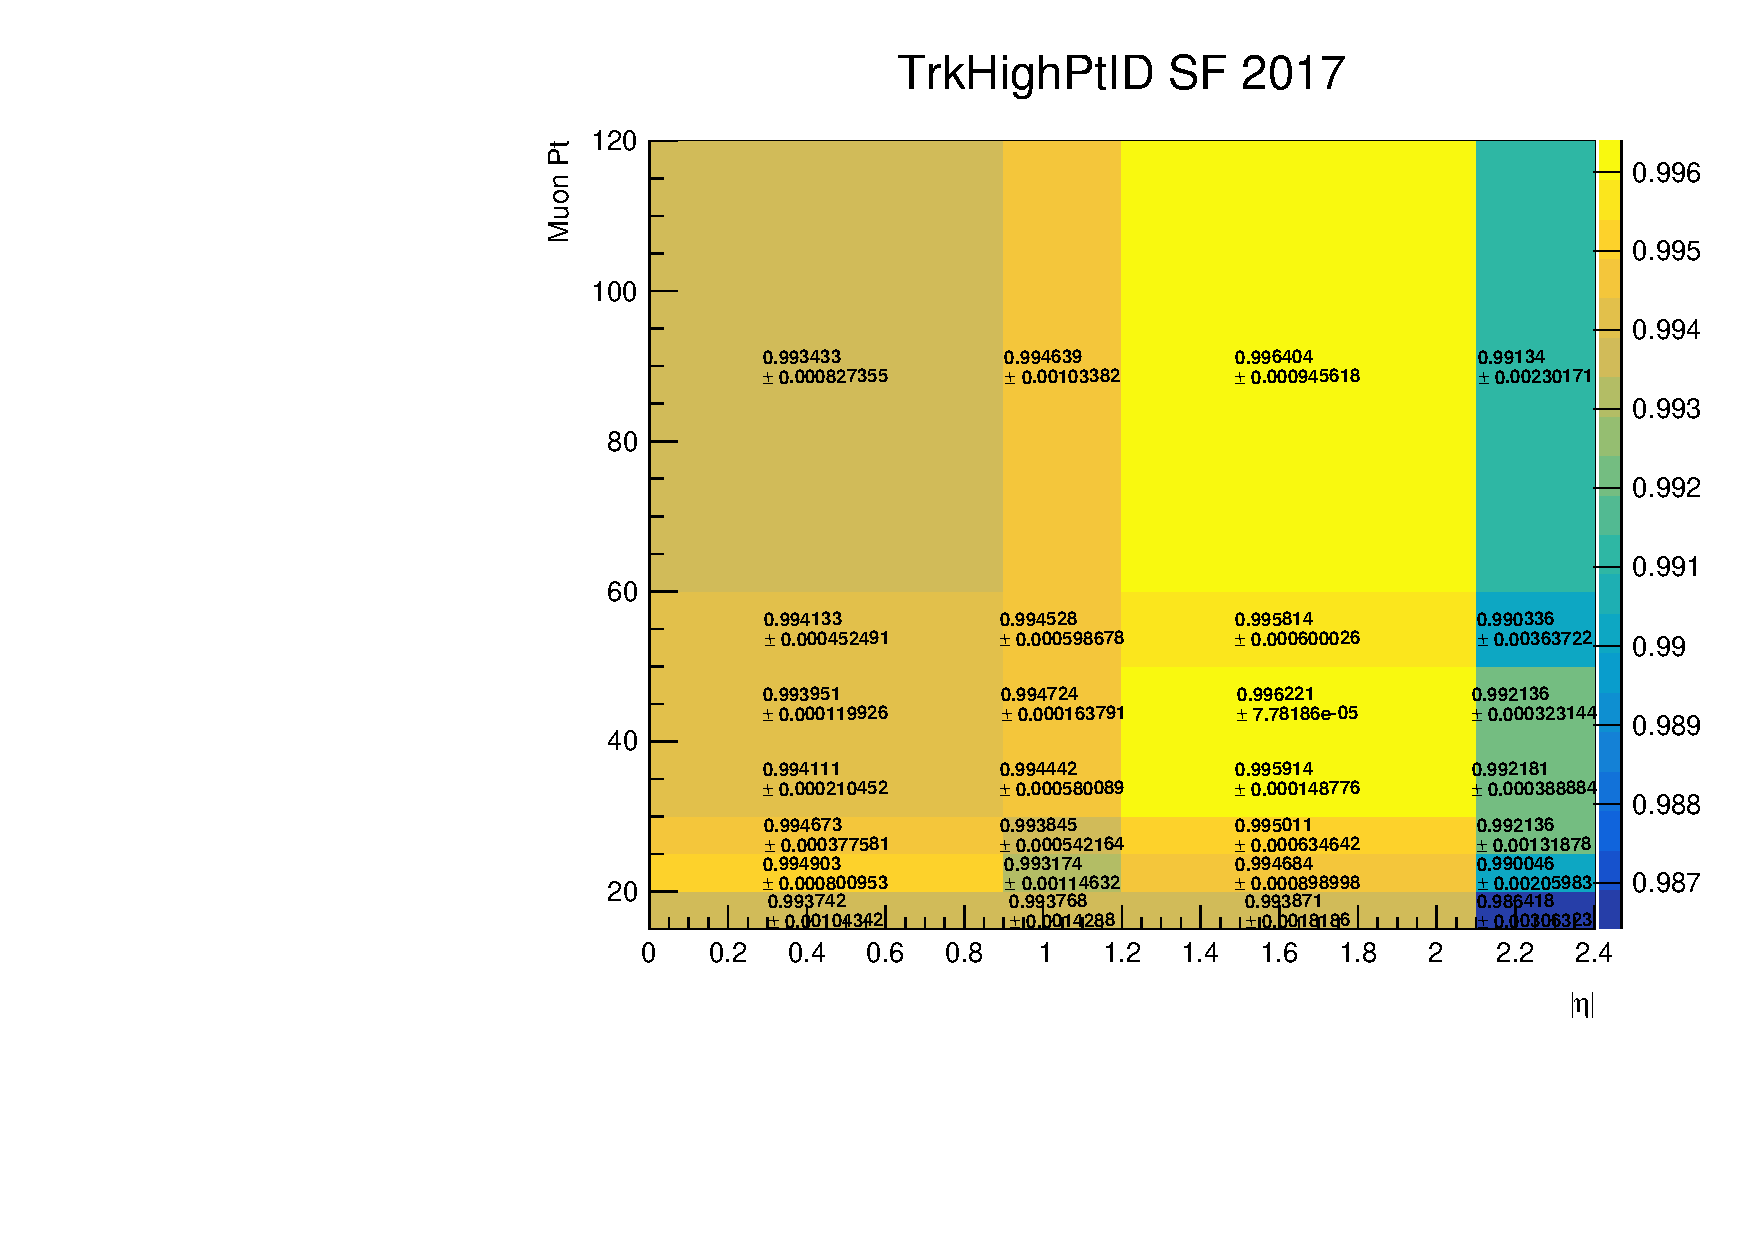
\includegraphics[width=.45\textwidth]{fig/ScaleFactors/2017Muon_TrkHighPtID.pdf}}
  \caption{Lepton ID Scale Factors 2017}
  \label{fig:leptonidsf_2017}
\end{figure}

\begin{figure}[tph]
  \centering
  \subfigure[Electron Loose ID. Applied to the $eee$ and $ee\mu$ channels
    based on the pseudorapidity $\eta$ and transverse momentum $P_{t}$ of each
    of the electrons used to define a $Z$ candidate in the event.
    The applied weight is the product of the scale factors of each individual electron.
  ]{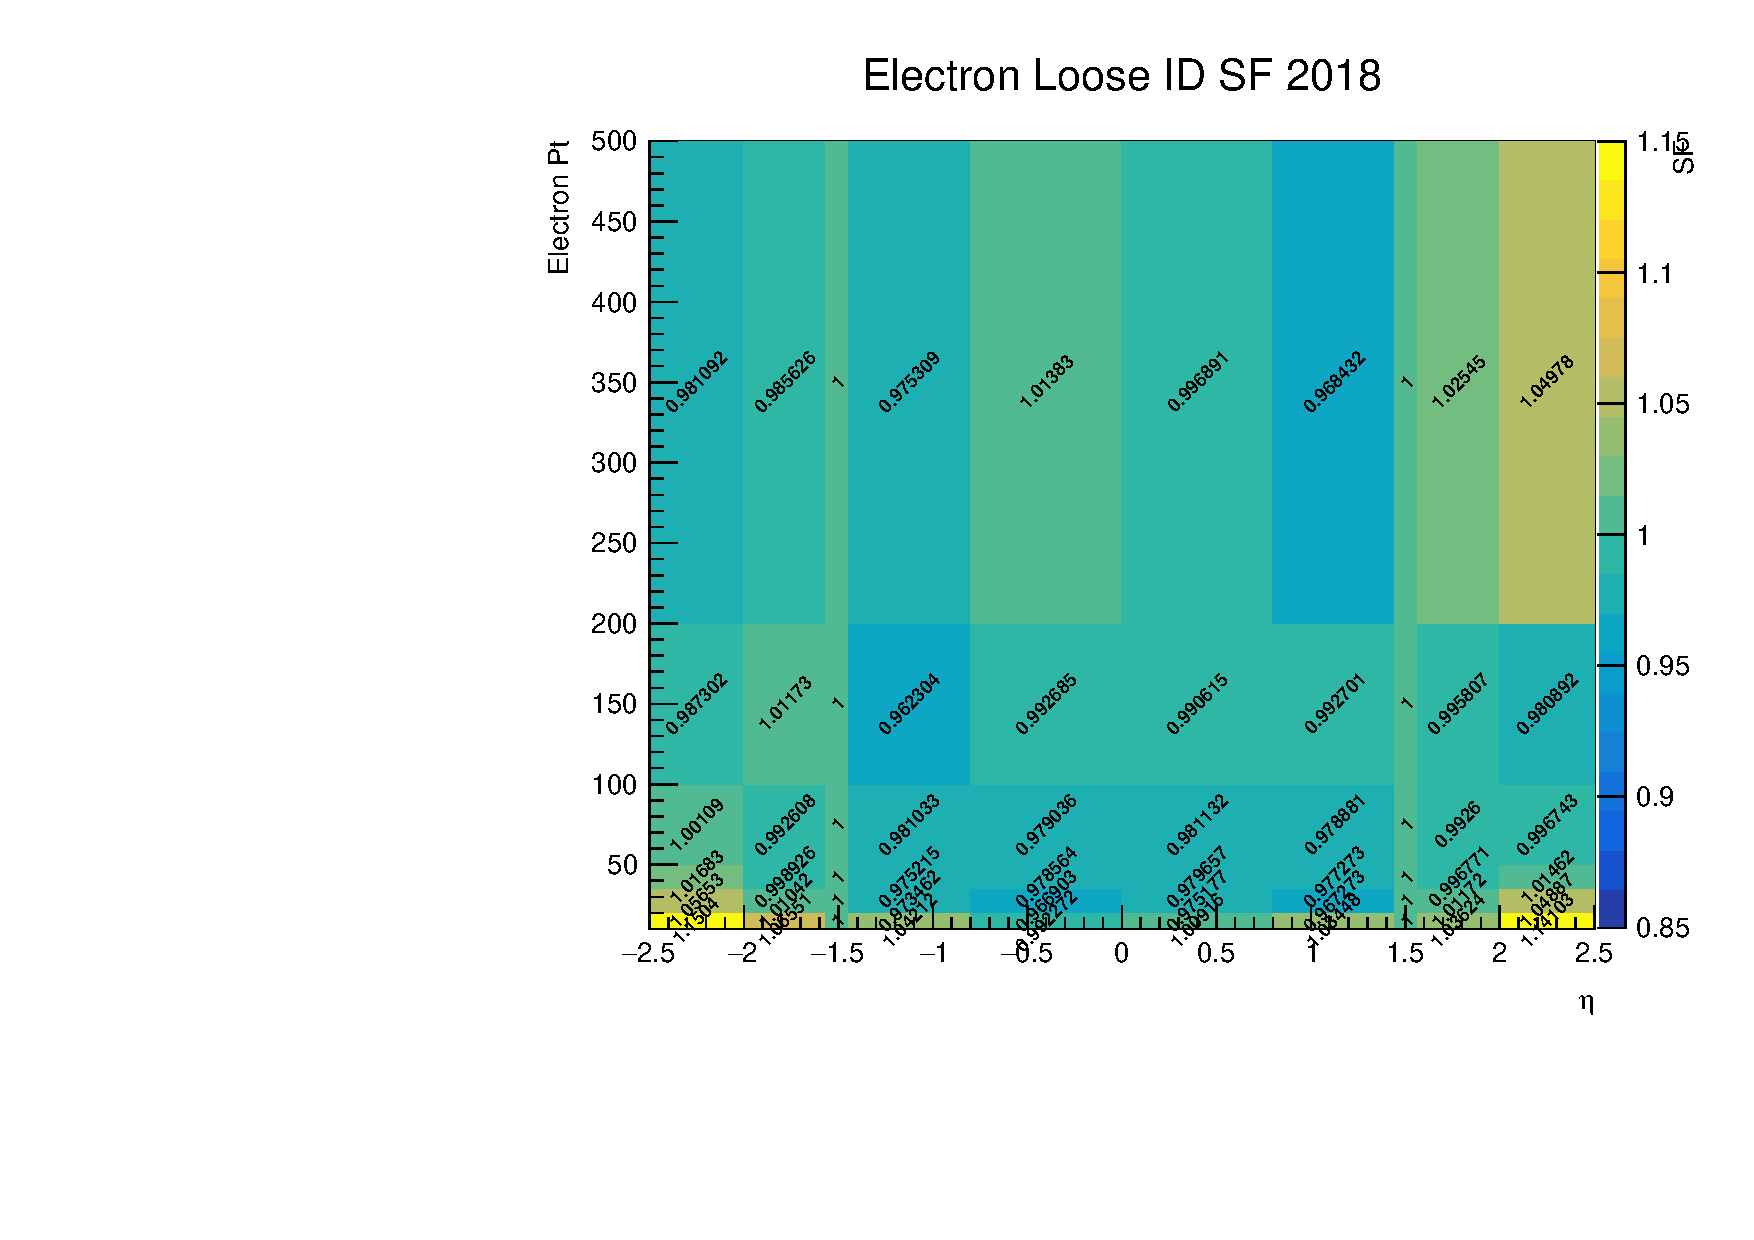
\includegraphics[width=.45\textwidth]{fig/ScaleFactors/2018Electron_LooseID.pdf}}
  \hspace{5mm}
  \subfigure[Electron Tight ID. Applied to the $eee$ and $\mu\mu e$ channels
    based on the pseudorapidity $\eta$ and transverse momentum $P_{t}$ of the
    electron used to define the $W$ candidate.]{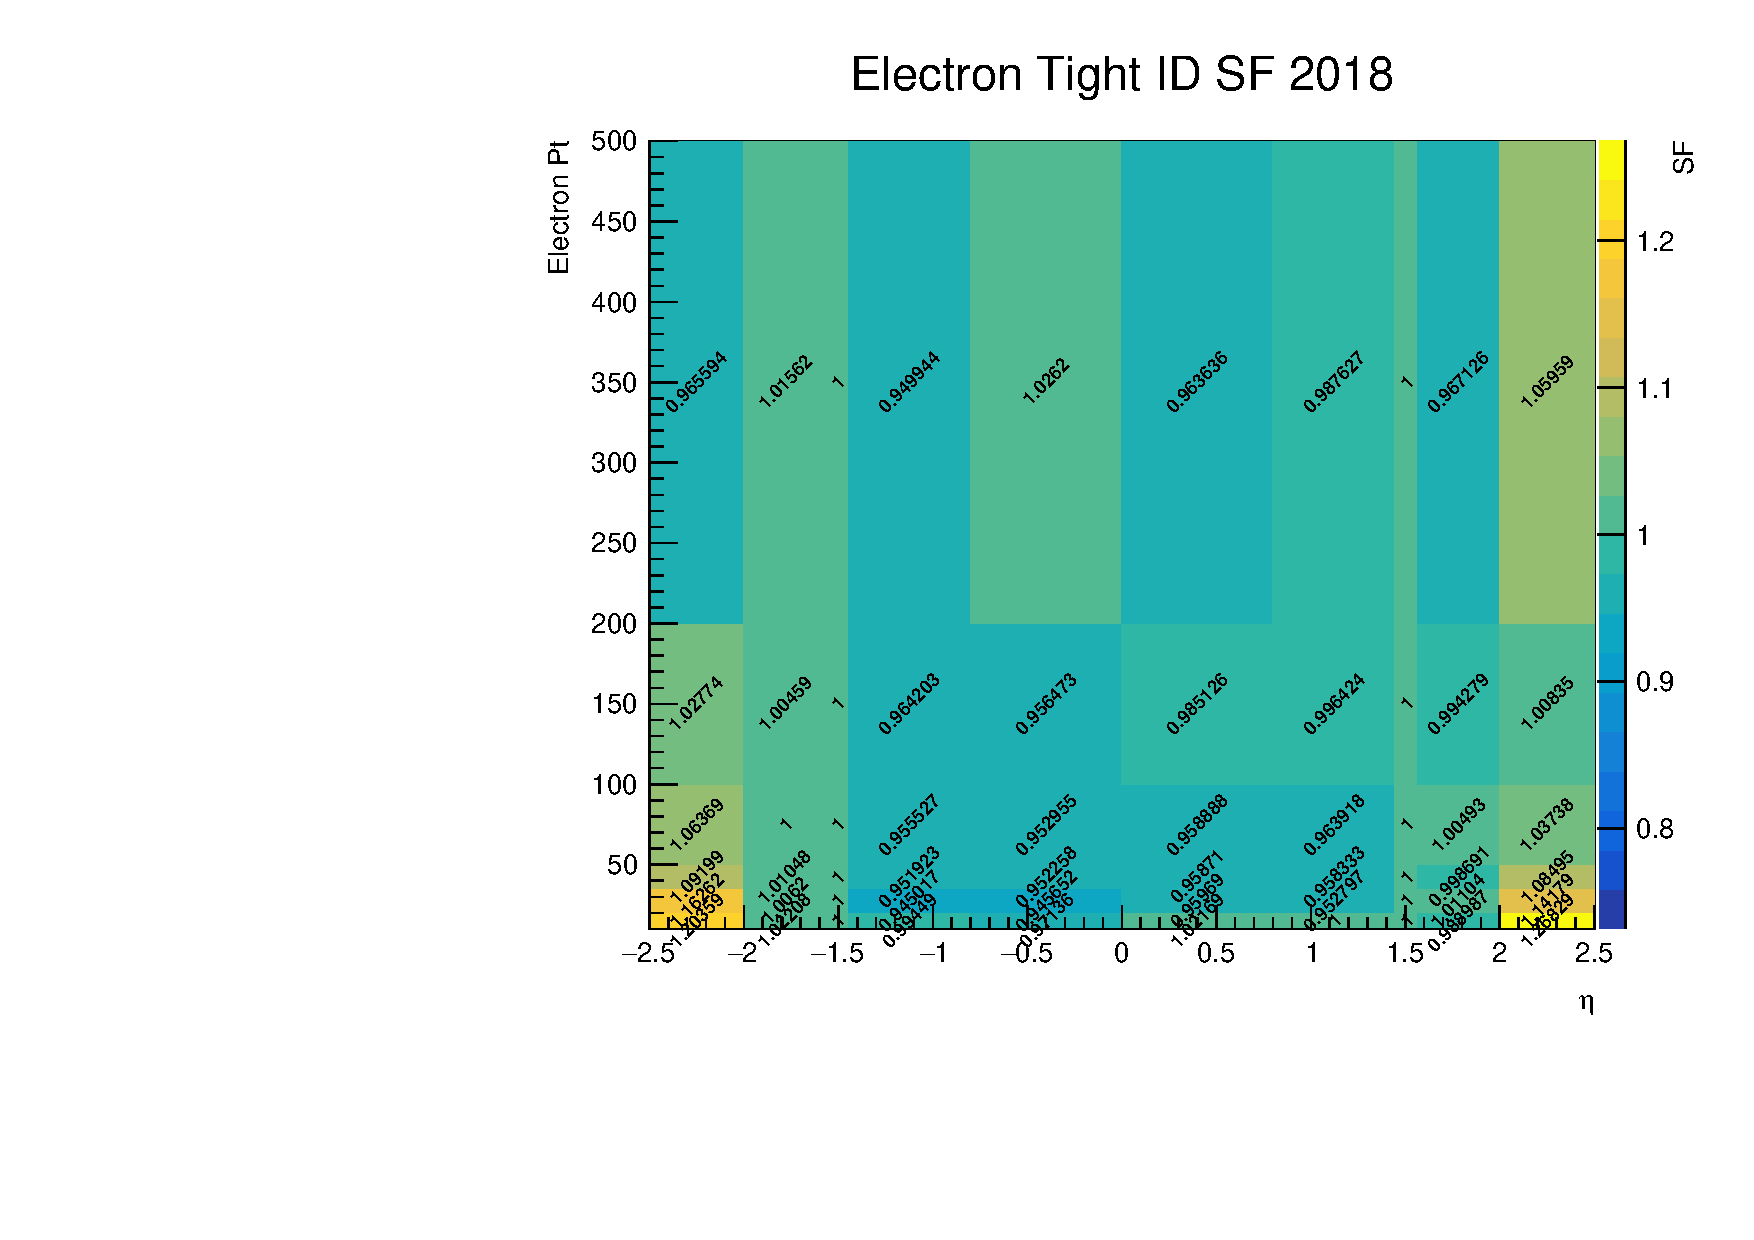
\includegraphics[width=.45\textwidth]{fig/ScaleFactors/2018Electron_TightID.pdf}}
  \vfil
  \subfigure[Muon GlobalHighPtId. Applied to the $\mu\mu e$, $ee\mu$,
    and $\mu\mu\mu$ channels based on the pseudorapidity $\eta$ and transverse
    momentum $P_{t}$ of each of the muons used to define a $WZ$ candidate in the event
    identified as GlobalHighPt.
    The applied weight is the product of the scale factors of each individual muon.
  ]{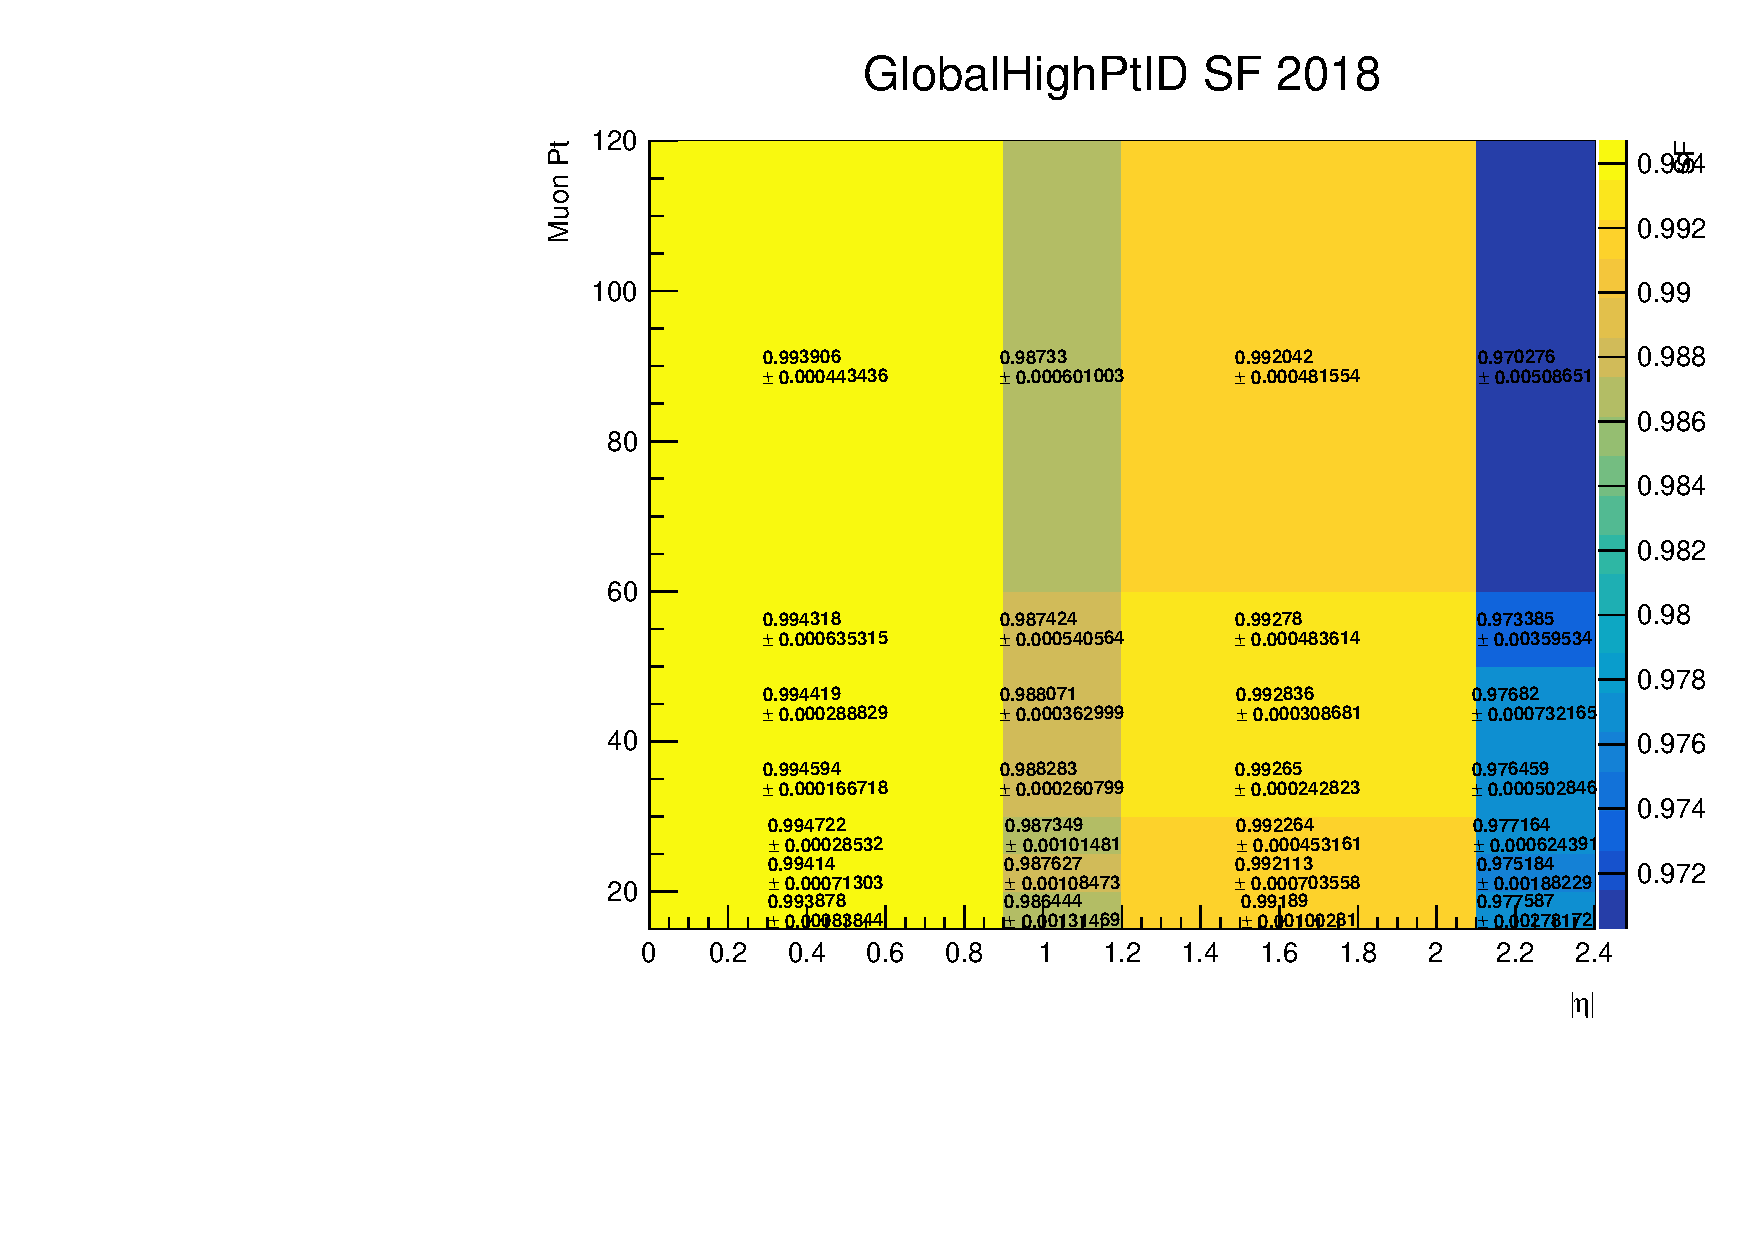
\includegraphics[width=.45\textwidth]{fig/ScaleFactors/2018Muon_GlobalHighPtID.pdf}}
  \hspace{5mm}
  \subfigure[Muon TrkHighPtId. Applied to the $\mu\mu e$ and $ee\mu$,
     and $\mu\mu\mu$ channels based on the pseudorapidity $\eta$ and transverse
     momentum $P_{t}$ of each of the muons used to define a $WZ$ candidate in the event
     identified as TrackerHighPt.
     The applied weight is the product of the scale factors of each individual muon.
  ]{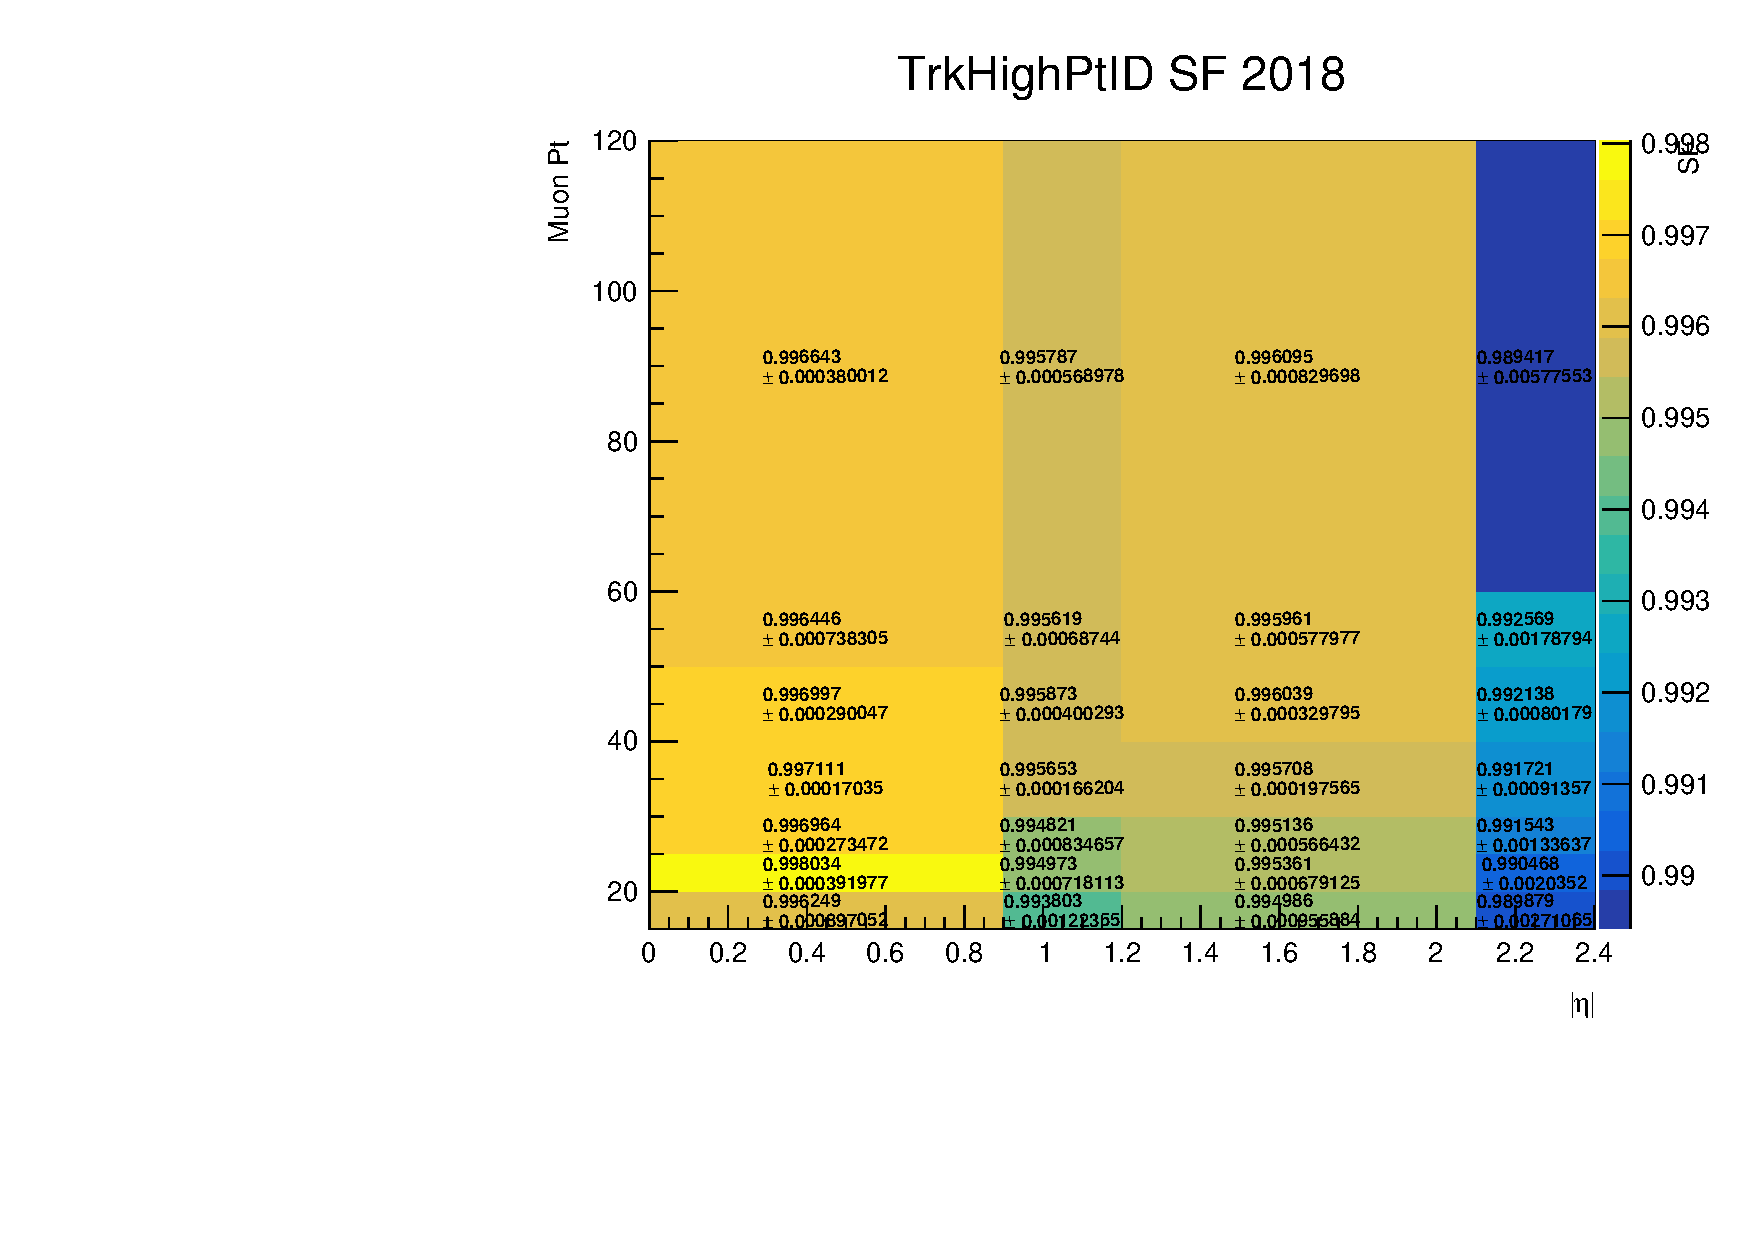
\includegraphics[width=.45\textwidth]{fig/ScaleFactors/2018Muon_TrkHighPtID.pdf}}
  \caption{Lepton ID Scale Factors 2018}
  \label{fig:leptonidsf_2018}
\end{figure}

Trigger and lepton identification efficiencies are different between data
and montecarlo. Scale factors are provided centrally by the Muon and EGamma POG
and show an $\eta-P_{t}$ dependence, see Figures \ref{fig:leptonidsf_2016},
\ref{fig:leptonidsf_2017}, and \ref{fig:leptonidsf_2018}.

The lepton identification scale factor is applied to the event
as a result of the product of each individual scale factor for each lepton in
the channel based on its transverse momentum $P_{t}$ and pseudorapidity $\eta$.
The HLT scale factor is applied based on the $P_{t}$ and $\eta$ of the leading
lepton: events corresponding to channels that include muons and electrons
will contain the product of the muon and electron HLT scale factor while events
from channels that include exclusively muon or electrons will be weighted with
the corresponding HLT scale factor.
Trigger and identification systematics are evaluated by moving up
and down the scale factors by their uncertainties. These uncertainties
are considered flat, independent of the resonance mass, and uncorrelated
in terms of lepton flavour.

